\documentclass[10pt,pdf,utf8,russian,aspectratio=169]{beamer}
\usepackage[T2A]{fontenc}
\usepackage[english,russian]{babel}
\usepackage{subfig}
\usepackage{amsmath}
\DeclareMathOperator*{\argmax}{arg\,max}
%
% Choose how your presentation looks.
%
% For more themes, color themes and font themes, see:
% http://deic.uab.es/~iblanes/beamer_gallery/index_by_theme.html
%
\mode<presentation>
{
  \usetheme{Boadilla}      % or try Darmstadt, Madrid, Warsaw, ...
  \usecolortheme{seagull} % or try albatross, beaver, crane, ..

  \usefonttheme{structurebold}  % or try serif, structurebold, ...
  \setbeamertemplate{navigation symbols}{}
  \setbeamertemplate{caption}[numbered]
} 

\captionsetup[subfloat]{labelformat=empty}
\title[Выбор моделей]{Выбор моделей глубокого обучения субпотимальной сложности}
\author{Бахтеев Олег}
\institute{МФТИ}
\date{14.03.2018}

\begin{document}

\begin{frame}
  \titlepage
\end{frame}

% Uncomment these lines for an automatically generated outline.
%\begin{frame}{План}
%  \tableofcontents
%\end{frame}

\section{Сложность модели}
\begin{frame}{Сложность модели: зачем?}
\begin{figure}
  \centering
  \subfloat[Устойчивость моделей при возмущении выборки]{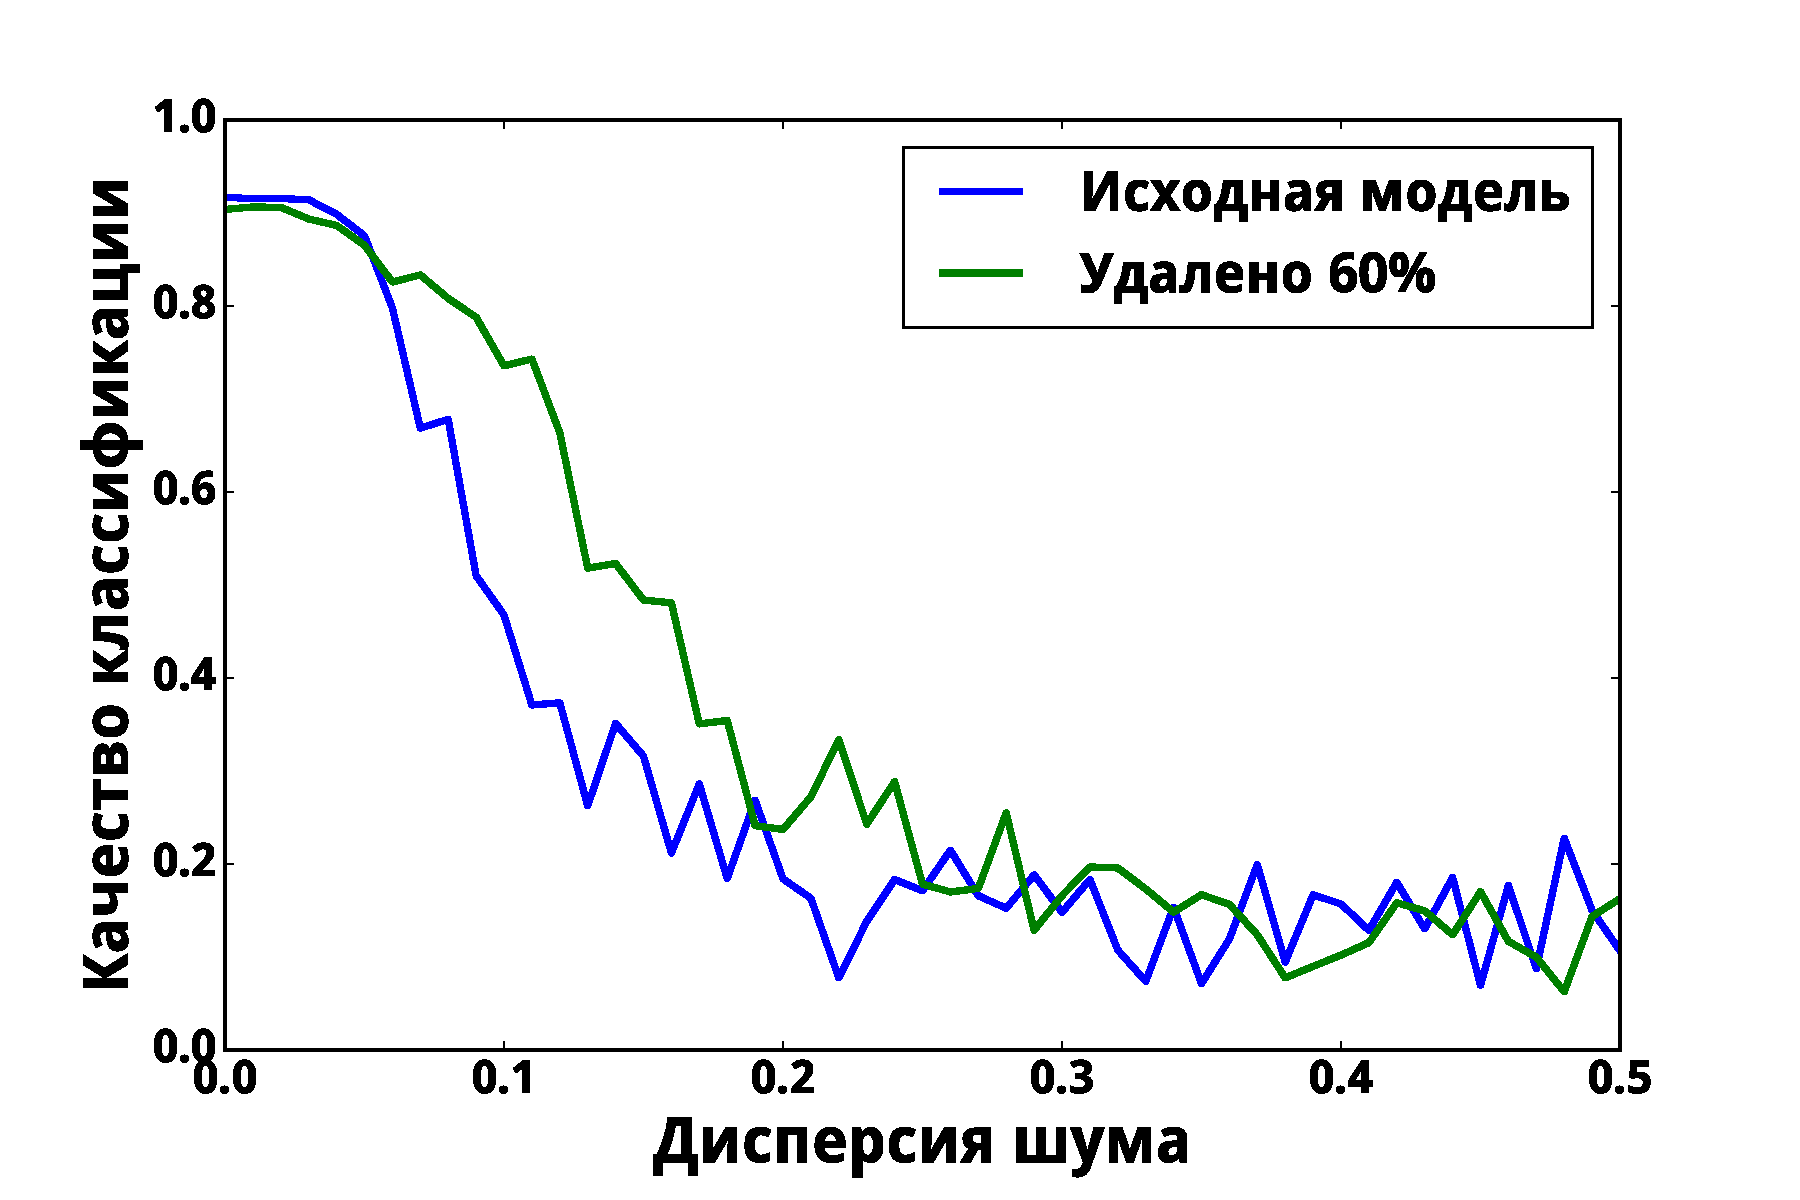
\includegraphics[width=0.4\textwidth]{noise.pdf}} 
 \subfloat[Качество классификации при удалении параметров]{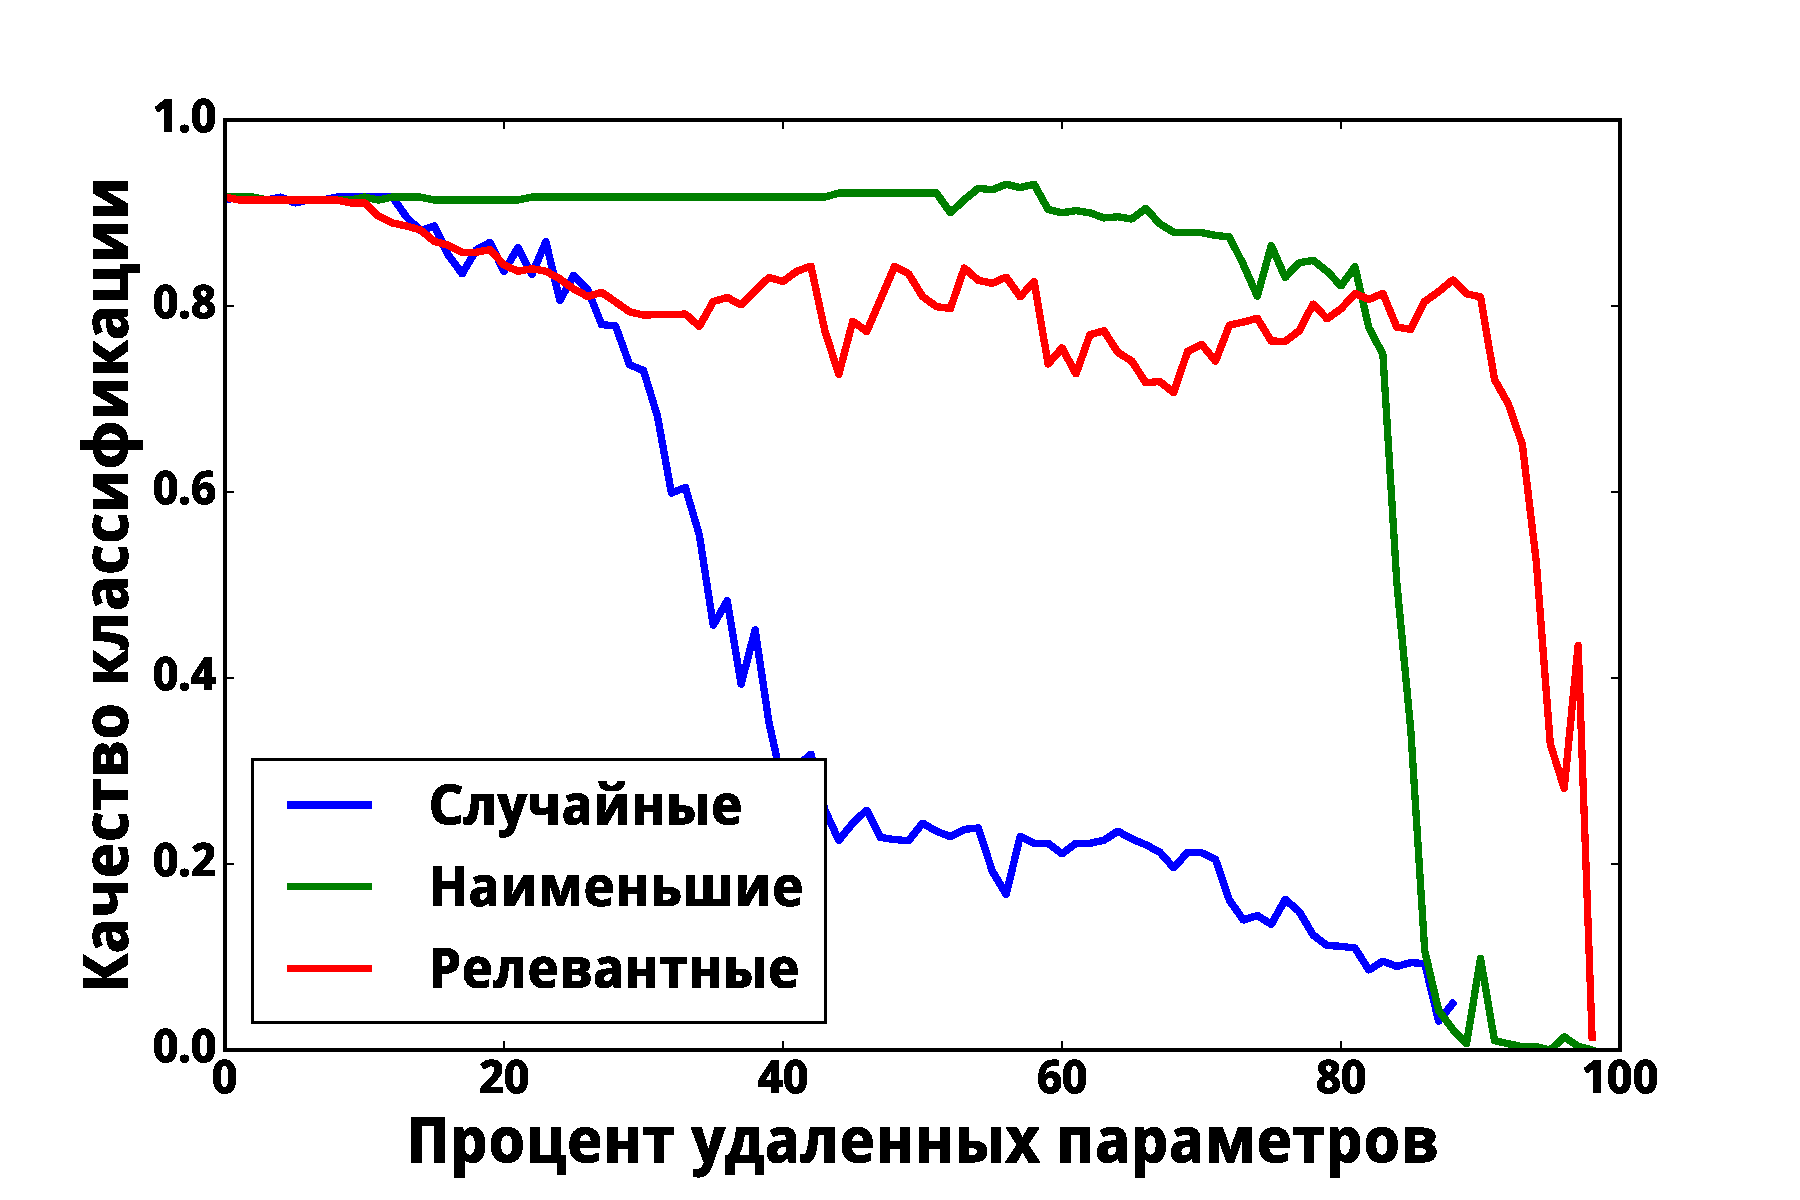
\includegraphics[width=0.4\textwidth]{pruning.pdf}}
\label{fig:1}\qquad

\end{figure}


\end{frame}

\begin{frame}{Сложность модели: зачем?}

\begin{figure}
  \centering
 {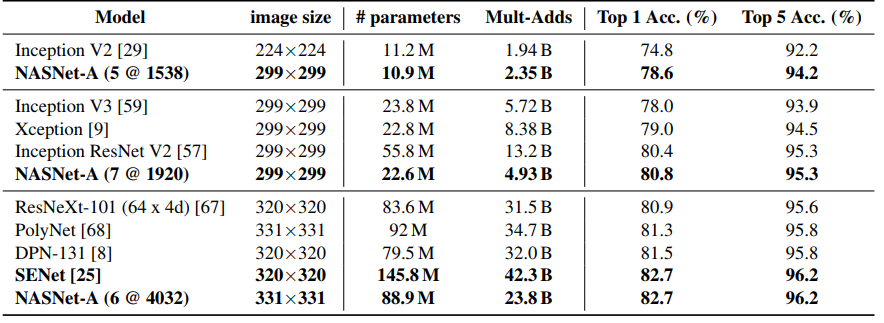
\includegraphics[width=\textwidth]{zoph.png}}
\label{fig:1}\qquad
\caption*{Zoph et. al, 2017.  Сложность моделей отличается почти в два раза при одинаковом качестве.}
\end{figure}
\end{frame}


\begin{frame}{Принцип минимальной длины описания}
\[
\text{MDL}(\mathbf{f}, \mathfrak{D}) = L(\mathbf{f}) + L(\mathfrak{D}|\mathbf{f}),
\]
где $\mathbf{f}$ --- модель, $\mathfrak{D}$ --- выборка, $L$ --- длина описания в битах.
\\
\[
\text{MDL}(\mathbf{f}, \mathfrak{D}) \sim L(\mathbf{f}) + L(\mathbf{w}^*| \mathbf{f}) + L(\mathfrak{D}|\mathbf{w}^*, \mathbf{f}),
\]
$\mathbf{w}^*$ --- оптимальные параметры модели.\\

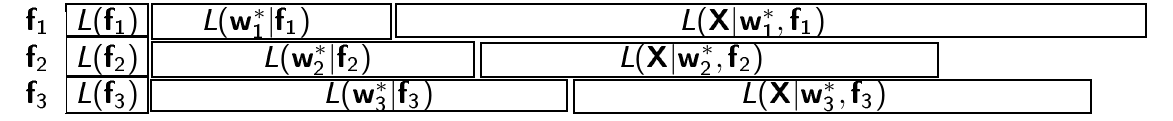
\includegraphics[width=\textwidth]{./mdl.png}

\end{frame}

\begin{frame}{MDL и Колмогоровская сложность}
\textbf{Колмогоровская сложность} --- длина минимального кода для выборки на предварительно заданном языке.

\textbf{Теорема инвариантности}\\
Для двух сводимых по Тьюрингу языков колмогоровская сложность  отличается не более чем на константу, не зависяющую от мощности выборки.\\

\textbf{Отличия от MDL}:
\begin{itemize}
\item Колмогоровская сложность невычислима.
\item Длина кода может зависеть от выбранного языка. Для небольших выборок теорема инвариантности не дает адекватных результатов.
\end{itemize}
\end{frame}

\begin{frame}{Оптимальная универсальная модель MDL}
Пусть выборка $\mathfrak{D}$ лежит в некотором конечном множестве $\mathbb{D}$.
%2.20
\[
\text{MDL}(\mathbf{f}, \mathfrak{D}) = L(\mathfrak{D}|\mathbf{w}^*(\mathfrak{D}), \mathbf{f}) + \text{COMP}(\mathbf{f}),
\]
$$ L(\mathfrak{D}|\mathbf{w}^*, \mathbf{f}) = -\text{log}p(\mathfrak{D}|\mathbf{w}^*(\mathfrak{D}), \mathbf{f}), \quad 
\text{COMP} = \text{log} \sum_{\mathfrak{D}' \in \mathbb{D}} p(\mathfrak{D}'|\mathbf{w}^*(\mathfrak{D}'), \mathbf{f}).$$

В случае, если распределение $p(\mathfrak{D}|\mathbf{w})$ принадлежит экспоненциальному семейству, оценка MDL совпадает с точностью до $o(1)$ с байесовской оценкой правдоподобия (``Evidence''):
\[
	p(\mathfrak{D}|\mathbf{f}) = \int_\mathbf{w} p(\mathfrak{D}|\mathbf{w})p(\mathbf{w}|\mathbf{f}) d\mathbf{w},
\]
где $p(\mathbf{w}|\mathbf{f})$ --- априорное распределение специального вида:
$$
	p(\mathbf{w}) = \frac{\sqrt{|J(\mathbf{w})|}}{\int_{\mathbf{w}'} \sqrt{|J(\mathbf{w'})|}d\mathbf{w'}},
$$
$J(\mathbf{w})$  --- информация Фишера.
\end{frame}	


\begin{frame}{Байесовый подход к сложности}
Правдоподобие модели (``Evidence''):
\[
	p(\mathfrak{D}|\mathbf{f}) = \int_\mathbf{w} p(\mathfrak{D}|\mathbf{w})p(\mathbf{w}|\mathbf{f}) d\mathbf{w}.
\]


\begin{figure}
  \centering
  \subfloat[Схема выбора модели по правдоподобию]{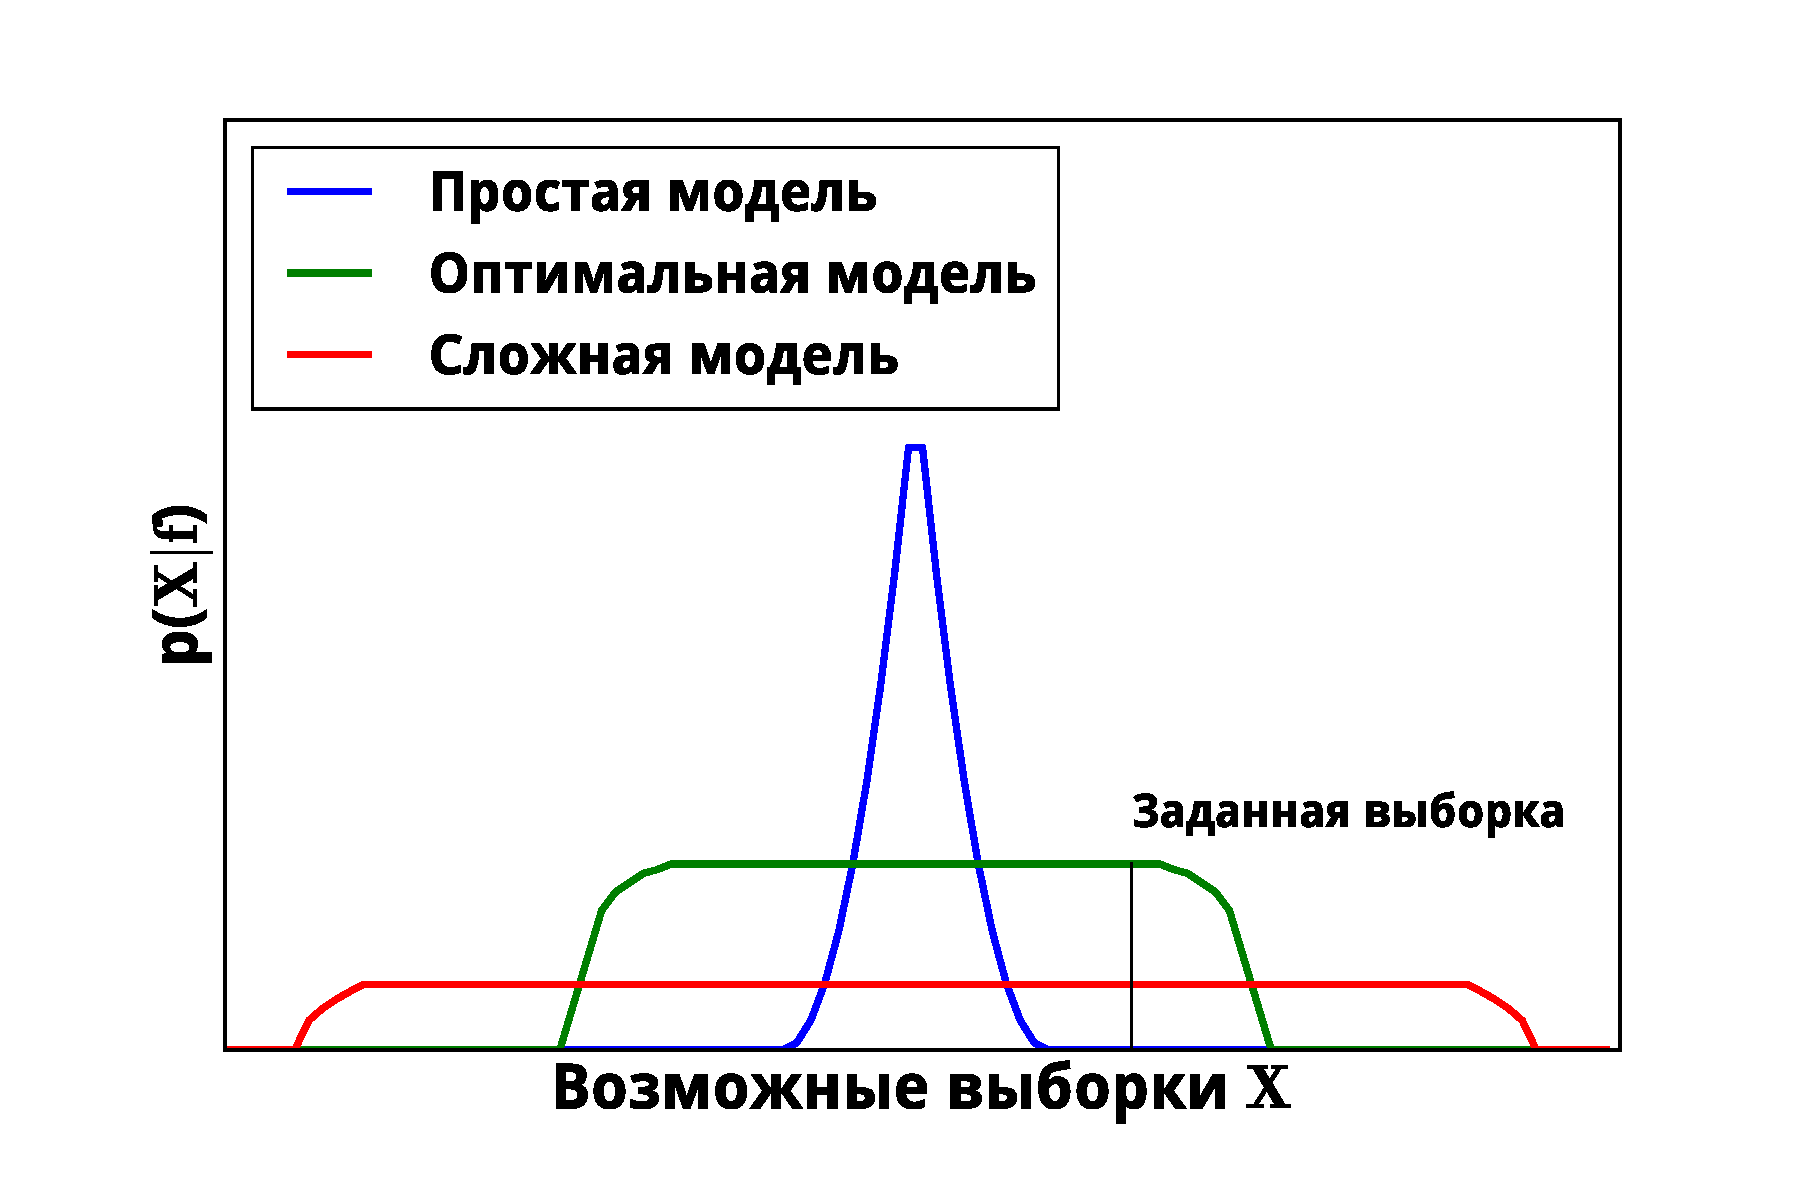
\includegraphics[width=0.4\textwidth]{evidence.pdf}} 
 \subfloat[Пример: полиномы]{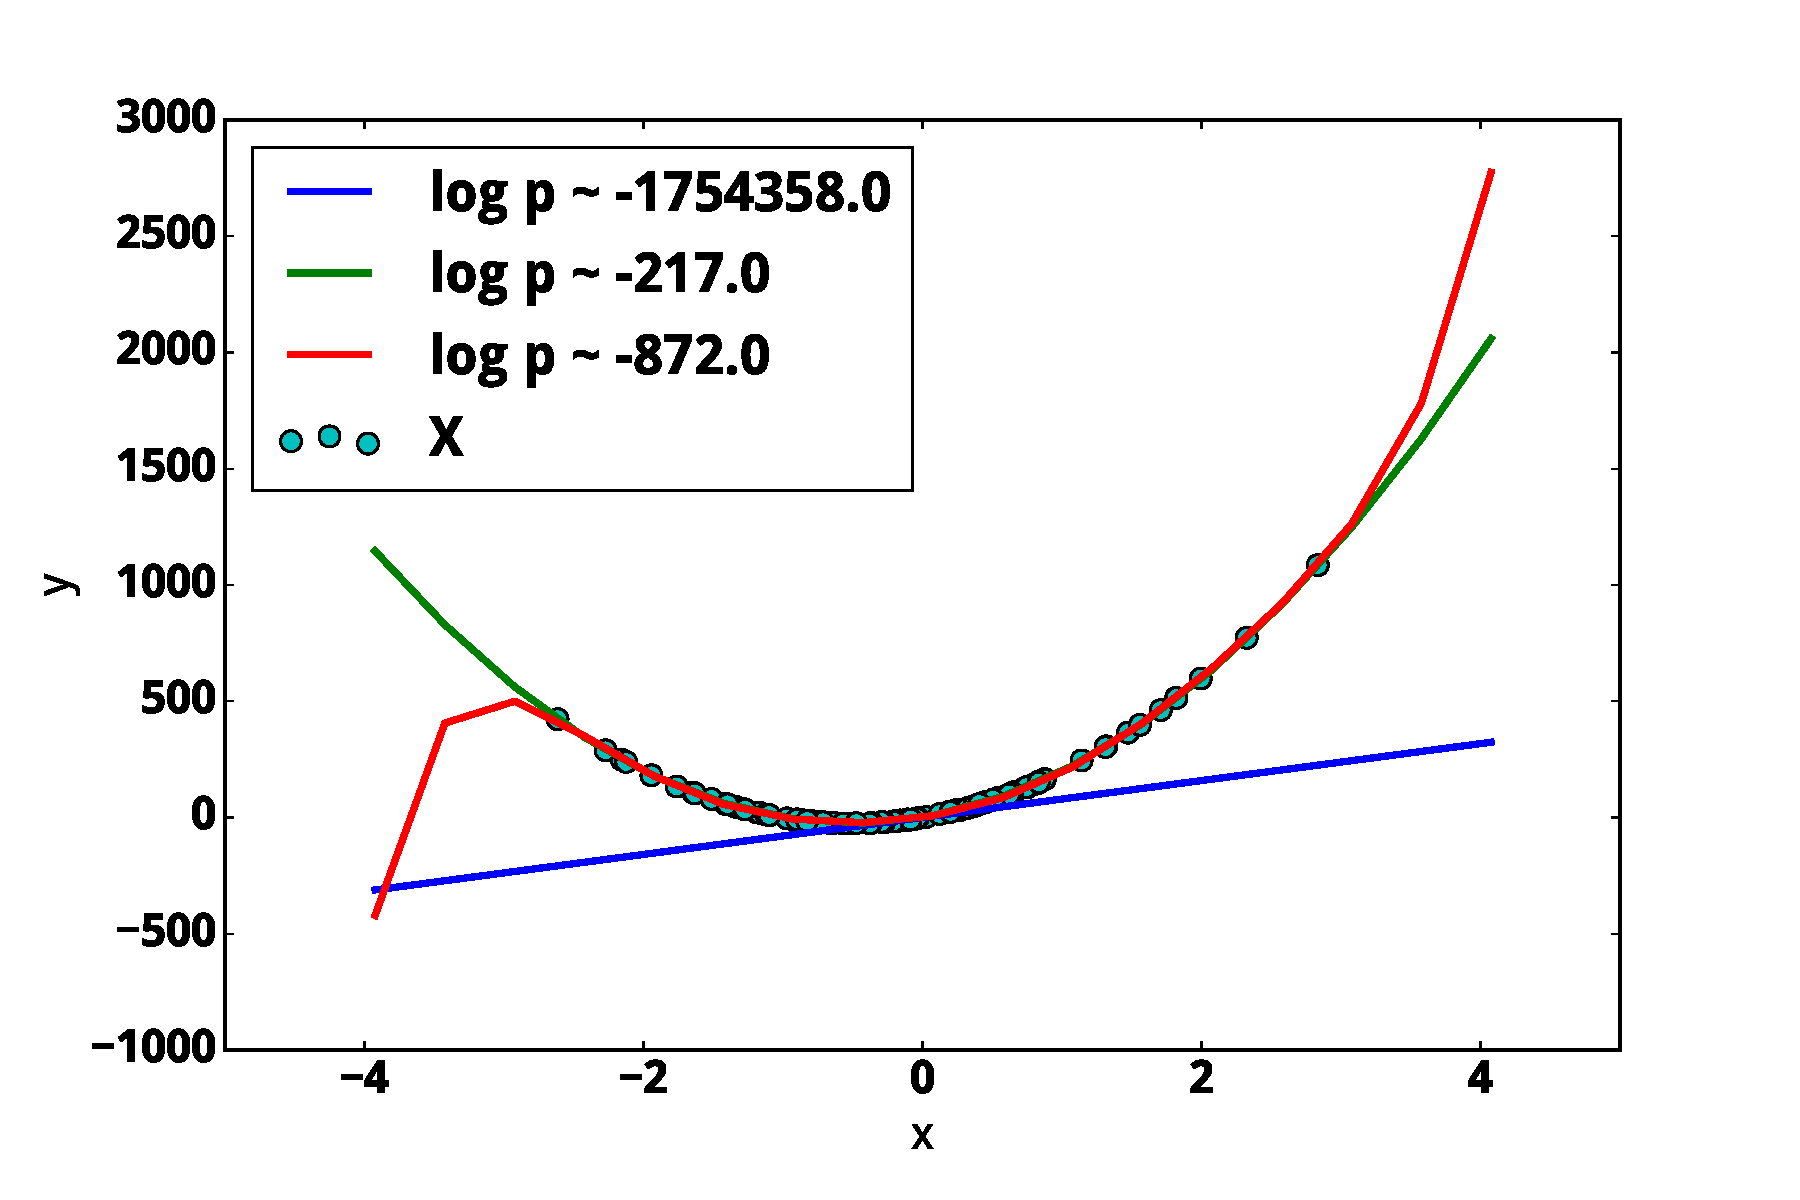
\includegraphics[width=0.4\textwidth]{example.pdf}}
\label{fig:1}\qquad

\end{figure}


\end{frame}

\begin{frame}{Evidence vs MDL}
\begin{tabular}{ c | c  }
  \hline			
 \bf Evidence & \bf MDL \\
  \hline  
Использует априорные знания &  Независима от априорных знаний \\
  \hline  
Основывается на гипотезе о порождении\\ выборки & Минимизирует длину описания выборки\\ вне зависимости от их природы \\
  \hline  

\end{tabular}


\begin{figure}
  \centering
 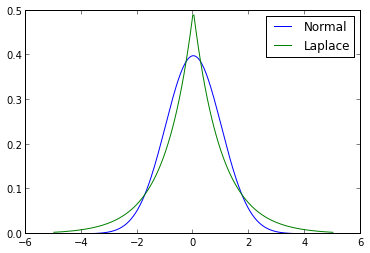
\includegraphics[width=0.4\textwidth]{laplace.png}
\label{fig:1}\qquad

\end{figure}


\end{frame}

\begin{frame}{Evidence vs Кросс-валидация}
Оценка Evidece:
\[
\text{log}~p(\mathfrak{D}|\mathbf{f}) = \text{log}~p(\mathfrak{D}_1|\mathbf{f}) + \text{log}~p(\mathfrak{D}_2|\mathfrak{D}_1, \mathbf{f}) + \dots +  \text{log}~p(\mathfrak{D}_n|\mathfrak{D}_1,\dots,\mathfrak{D}_{n-1}, \mathbf{f}).
\]

Оценка leave-one-out:
\[
\text{LOU} = \mathsf{E} \text{log}~p(\mathfrak{D}_n|\mathfrak{D}_1,\dots,\mathfrak{D}_{n-1}, \mathbf{f}).
\]

Кросс-валидация использует среднее значение последнего члена $p(\mathfrak{D}_n|\mathfrak{D}_1,\dots,\mathfrak{D}_{n-1}, \mathbf{f})$ для оценки сложности. \\
Evidence учитывает \textbf{полную} сложность описания заданной выборки, определяющую предсказательную способность модели с самого начала.
\end{frame}


\begin{frame}{Оптимальность модели}
\begin{block}{Определение}
Пусть задано множество моделей $\mathfrak{F}$.  \\
Пусть для каждой модели $\mathbf{f}$ задано априорное распределение параметров: $p(\mathbf{w}|\mathbf{f})$.\\
Модель $\mathbf{f}$ назовем оптимальной среди моделей $\mathfrak{F}$, если достигается максимум интеграла:
\[
	p(\mathfrak{D}|\mathbf{f}) = \int_\mathbf{w} p(\mathfrak{D}|\mathbf{w})p(\mathbf{w}|\mathbf{f}) d\mathbf{w}.
\]
\end{block}
\end{frame}

\begin{frame}{Пример: линейная регрессия}
Рассмотрим задачу линейной регрессии:
\[
	\mathbf{y} =\mathbf{X} \mathbf{w} + \boldsymbol{\varepsilon},\quad \boldsymbol{\varepsilon}  \sim \mathcal{N}(\mathbf{0},\mathbf{1}),\quad \mathbf{w} \sim  \mathcal{N}(\mathbf{0},\mathbf{A}^{-1}),\quad  \mathbf{X} \in \mathbb{R}^{m \times n},
\]
где $\mathbf{A}$ --- диагональная матрица. 

\[
	p(\mathbf{y}|  \mathbf{X}, \mathbf{w}, \mathbf{f}) = (2\pi) ^{-\frac{m}{2}} \textnormal{exp} \bigl(-\frac{1}{2}(\mathbf{y} -\mathbf{X} \mathbf{w})^\mathsf{T}(\mathbf{y} - \mathbf{X}\mathbf{w})\bigr),
\quad
p(\mathbf{w}|\mathbf{f}) =  (2\pi) ^{-\frac{n}{2}} |\mathbf{A}|^{\frac{1}{2}} \textnormal{exp} (-\frac{1}{2}\mathbf{w}^\mathsf{T}\mathbf{A}\mathbf{w}).
\]
Правдоподобие модели $p(\mathfrak{D}|\mathbf{f})$ вычисляется аналитически:
\[
	p(\mathfrak{D}|\mathbf{f})  =  (2\pi) ^{-\frac{m}{2}} |\mathbf{A}|^{\frac{1}{2}} |\mathbf{H}|^{-\frac{1}{2}}  \textnormal{exp}\bigl(-\frac{1}{2}(\mathbf{y} -\mathbf{X} \hat{\mathbf{w}})^\mathsf{T}(\mathbf{y} - \mathbf{X}\hat{\mathbf{w}})\bigr)\textnormal{exp} \bigl(-\frac{1}{2}\hat{\mathbf{w}}^\mathsf{T}\mathbf{A}\hat{\mathbf{w}}\bigr),
\]

где $\hat{\mathbf{w}}$ --- значение наиболее вероятных параметров модели:
\[
	\hat{\mathbf{w}} = \argmax p(\mathbf{w}|\mathbf{y}, \mathbf{X}, \mathbf{f}) = (\mathbf{A} + \mathbf{X}^\mathsf{T}\mathbf{X})^{-1}\mathbf{X}^\mathsf{T}\mathbf{y},
\]
$\mathbf{H}$ --- гессиан функции потерь $- \textnormal{log} p(\mathbf{y}|  \mathbf{X}, \mathbf{w}, \mathbf{f})$:
\[
	\mathbf{H}	= \nabla \nabla_\mathbf{w} \left(\frac{1}{2} (\mathbf{y} -\mathbf{X} {\mathbf{w}})^\mathsf{T}(\mathbf{y} - \mathbf{X}{\mathbf{w}}) + \frac{1}{2}\mathbf{w}^\mathsf{T}\mathbf{A}\mathbf{w} \right) = \mathbf{A} + \mathbf{X}^\mathsf{T}\mathbf{X}.
\]


\end{frame}

\begin{frame}{Методы получения оценок Evidence: метод Лапласа}
$$
	p(\mathfrak{D}|\mathbf{f}) = \int_\mathbf{w} p(\mathfrak{D}|\mathbf{w}) p(\mathbf{w}|\mathbf{f}) = \int_\mathbf{w} \text{exp}(-S(\mathbf{w}))	\sim  \text{exp}\bigl(S(\hat{\mathbf{w}})\bigr) \int_\mathbf{w} \text{exp} (-\frac{1}{2}\Delta \mathbf{w}^\text{T} \nabla \nabla S(\hat{\mathbf{w}}) \Delta \mathbf{w} ).
$$

\begin{figure}
  \centering
 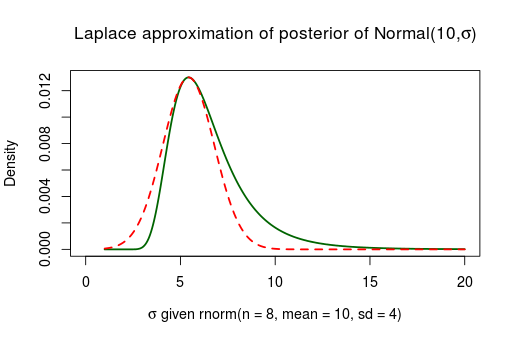
\includegraphics[width=0.4\textwidth]{laplace2.png}
\label{fig:1}\qquad	
\end{figure}

\end{frame}
\begin{frame}{Методы получения оценок Evidence: Метод Монте-Карло}
$$
p(\mathfrak{D}|\mathbf{f})  \sim \frac{1}{K}\sum_{\mathbf{w} \in \mathbf{W}} p(\mathfrak{D}|\mathbf{w},\mathbf{f})p(\mathbf{w}|\mathbf{f}),
$$
$\mathbf{W}$ --- множество векторов параметров мощностью $K$.

\begin{itemize}
\item Плохо работает в пространствах большой размерности
\item Существует ряд модификаций, позволяющих преодолеть проклятие размерности
\item Может применяться в связке с вариационным выводом
\end{itemize}
\end{frame}


\section{Вариационная нижняя оценка}
\begin{frame}{Вариационная оценка}
%http://www.orchid.ac.uk/eprints/40/1/fox_vbtut.pdf
\textbf{Вариационная оценка Evidence} --- метод нахождения приближенного значения аналитически невычислимого распределения $p(\mathbf{w}|\mathfrak{D}, \mathbf{f})$ распределением $q(\mathbf{w}) \in \mathbf{Q}$. Получение вариационной нижней оценки обычно сводится к задаче минимизации
$$\text{KL}(q(\mathbf{w})||p(\mathbf{w}| \mathfrak{D}))=
-\int_{\mathbf{w}} q(\mathbf{w}) \text{log}~\frac{p(\mathbf{w}| \mathfrak{D})} {q(\mathbf{w})}d\mathbf{w}.
$$

\begin{figure}
  \centering
  \subfloat[Аппроксимация неизвестного распределения нормальным]{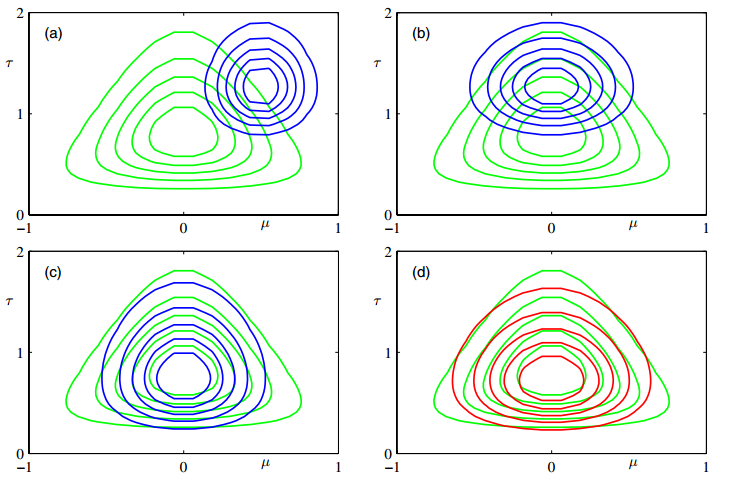
\includegraphics[width=0.33\textwidth]{omnomnom.png}} 
 \subfloat[Аппроксимация Лапласа (красная линия) и вариационная оценка (зеленая линия)]{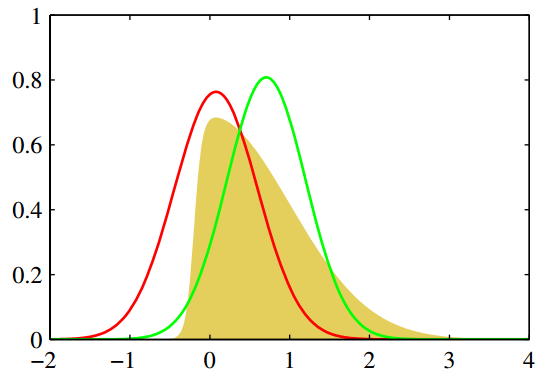
\includegraphics[width=0.33\textwidth]{laplace_vs_var.png}}
\label{fig:1}\qquad

\end{figure}

\end{frame}

\begin{frame}{Получение вариацонной нижней оценки}
$$
\text{log}~p(\mathfrak{D}| \mathbf{f})  = \int_{\mathbf{w}} q(\mathbf{w})\text{log}~\frac{p(\mathfrak{D},\mathbf{w}|\mathbf{f})}{q(\mathbf{w})}d\mathbf{w} + \text{D}_\text{KL}  (q(\mathbf{w})||p(\mathbf{w}| \mathfrak{D}, \mathbf{f})) \geq	
$$
$$
\geq \int_{\mathbf{w}} q(\mathbf{w})\text{log}~\frac{p(\mathfrak{D},\mathbf{w}|\mathbf{f})}{q(\mathbf{w})}d\mathbf{w} =
$$

$$
= -\text{D}_\text{KL} (q(\mathbf{w})||p(\mathbf{w}|\mathbf{f})) + \int_{\mathbf{w}} q(\mathbf{w})\text{log}~{p(\mathfrak{D}|\mathbf{w},\mathbf{f})} d \mathbf{w},
$$
где $$\text{D}_\text{KL}(q(\mathbf{w})||p(\mathbf{w} |\mathbf{f})) = -\int_{\mathbf{w}} q(\mathbf{w})\text{log}~\frac{p(\mathbf{w} | \mathbf{f})}{q(\mathbf{w})}d\mathbf{w}.$$
\begin{block}{Определение} Модель $\mathbf{f}$ назовем субоптимальной на множестве моделей $\mathfrak{F}$  по множеству распределений ${Q}$, если модель доставляет максимум нижней вариационной оценке:
\[
\label{eq:elbo2}
	\mathbf{f} = \argmax_{\hat{\mathbf{f}} \in \mathfrak{F}}\max_{q \in {Q}}\int_{\mathbf{w}} q(\mathbf{w})\textnormal{log}~\frac{p(\mathbf{y},\mathbf{w}|\mathfrak{D},\hat{\mathbf{f})}}{q(\mathbf{w})}d\mathbf{w}.
\]
\end{block}


\end{frame}

\begin{frame}{$D_\text{KL}$}
Максимизация вариационной нижней оценки $$\int_{\mathbf{w}} q(\mathbf{w})\text{log}~\frac{p(\mathfrak{D},\mathbf{w}|\mathbf{f})}{q(\mathbf{w})}d\mathbf{w}$$   эквивалентна минимизации дивергенции между распределением распределением $q(\mathbf{w}) \in Q$ и апостериорным распределением параметров $p(\mathbf{w}|\mathfrak{D}, \mathbf{f})$:
\[
q = \text{argmax}_{q \in Q}\int_{\mathbf{w}} q(\mathbf{w})\text{log}~\frac{p(\mathfrak{D},\mathbf{w}|\mathbf{f})}{q(\mathbf{w})}d\mathbf{w} \Leftrightarrow 	
q = \text{argmin}_{q \in Q} \text{D}_\text{KL}  (q(\mathbf{w})||p(\mathbf{w}| \mathfrak{D}, \mathbf{f})),
\]
т.к.
$$\text{log}~p(\mathfrak{D}| \mathbf{f})  = \int_{\mathbf{w}} q(\mathbf{w})\text{log}~\frac{p(\mathfrak{D},\mathbf{w}|\mathbf{f})}{q(\mathbf{w})}d\mathbf{w} + \text{D}_\text{KL}  (q(\mathbf{w})||p(\mathbf{w}| \mathfrak{D}, \mathbf{f})) = \text{const}.$$



\end{frame}

\begin{frame}{Пример: аппроксимация мультимодального распределения}
Вместо минимизации $\text{D}_\text{KL} (q(\mathbf{w})||p(\mathbf{w}|\mathbf{f}))$ можно также минимизировать $\text{D}_\text{KL} (p(\mathbf{w}|\mathbf{f})||q(\mathbf{w}))$. Метод, основанный на данной оптимизации, называется Expectation Propagation (рис. слева).

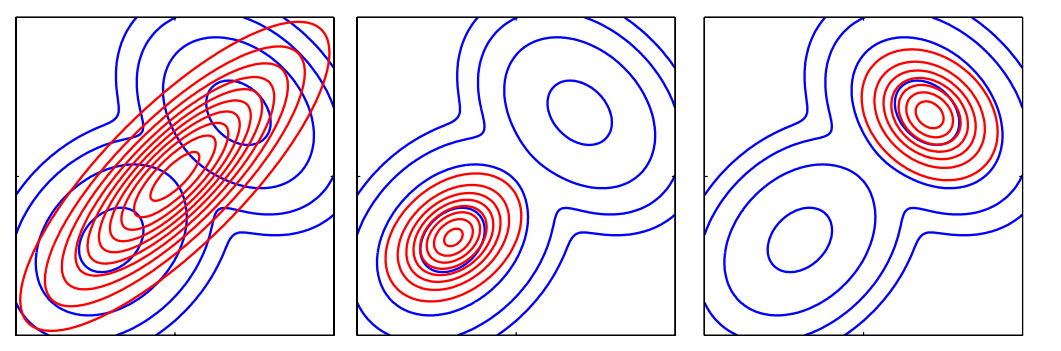
\includegraphics[width=\textwidth]{bishop.png}

\end{frame}



\begin{frame}{Использование вариационной нижней оценки}
\textbf{Для чего используют вариационный вывод?}
\begin{itemize}
\item получение оценок Evidence;
\item получение оценок распределений моделей со скрытыми переменными (тематическое моделирование, снижение размерности).
\end{itemize}

\textbf{Зачем используют вариационный вывод?}
\begin{itemize}
\item сводит задачу нахождения апостериорной вероятности к методам оптимизации;
\item проще масштабируется, чем аппроксимация Лапласа;
\item проще в использовании, чем сэмплирующие методы.
\end{itemize}
\textbf{Вариационный вывод может давать сильно заниженную оценку.}
\end{frame}


\section{Получение оценок для разделяющих моделей}
\begin{frame}{Evidence: нормальное распределение}
Пусть $q \sim \mathcal{N}(\boldsymbol{\mu}_q, \mathbf{A}_q).$\\
Тогда вариационная оценка имеет вид:
$$
\int_{\mathbf{w}} q(\mathbf{w})\text{log}~{p(\mathbf{Y}|\mathbf{X},\mathbf{w},\mathbf{f})} d \mathbf{w} - D_\text{KL}\bigl(q (\mathbf{w} )|| p (\mathbf{w}|\mathbf{f})\bigr) \simeq
$$
$$
\sum_{i=1}^m \text{log}~p(\mathbf{y}_i|\mathbf{x}_i, \hat{\mathbf{w}}) - D_\text{KL}\bigl(q (\mathbf{w} )|| p (\mathbf{w}|\mathbf{f})\bigr) \to \max_{\mathbf{A}_q, \boldsymbol{\mu}_q}, \quad \hat{\mathbf{w}} \sim q.
$$
В случае, если априорное распределение параметров $p(\mathbf{w}|\mathbf{f})$ является нормальным: 
$$
p(\mathbf{w}|\mathbf{f}) \sim \mathcal{N}(\boldsymbol{\mu}, \mathbf{A}),
$$
дивергенция $D_\text{KL}\bigl(q (\mathbf{w} )|| p (\mathbf{w}|\mathbf{f})$ вычисляется аналитически:
$$
D_\text{KL}\bigl(q (\mathbf{w}) || p (\mathbf{w}|\mathbf{f})\bigr) = \frac{1}{2} \bigl( \text{tr} (\mathbf{A}^{-1}\mathbf{A}_q) + (\boldsymbol{\mu} - \boldsymbol{\mu}_q)^\text{T}\mathbf{A}^{-1}(\boldsymbol{\mu} - \boldsymbol{\mu}_q) - n +\text{ln}~|\mathbf{A}| - \text{ln}~|\mathbf{A}_q| \bigr).
$$
\end{frame}



\begin{frame}{Evidence: нормальное распределение}
\begin{columns}[T] 
\begin{column}{.48\textwidth}
\textbf{``Обычная'' функция потерь:}\\
$$
L = \textcolor{red}{\sum_{\mathbf{x}, \mathbf{y} \in \mathfrak{D}} - \text{log}p(\mathbf{y}|\mathbf{x}, \mathbf{w})} + \textcolor{blue}{\lambda||\mathbf{w}||_2^2}.
$$\\~\\

% если n - константна.
\textbf{Вариационный вывод при $(p(\mathbf{w}|\mathbf{f}) \sim \mathcal{N}(\mathbf{0}, \mathbf{1}))$:}\\
$$
L =   \textcolor{red}{\sum_{\mathbf{x}, \mathbf{y}} \text{log}~p(\mathbf{y}|\mathbf{x}, \hat{\mathbf{w}})} +
$$
$$ + \textcolor{blue}{\frac{1}{2} \bigl( \text{tr} (\mathbf{A}_q) + \boldsymbol{\mu}_q^\text{T}\mathbf{A}^{-1}\boldsymbol{\mu}_q  - \text{ln}~|\mathbf{A}_q| \bigr)}.
$$\\~\\

\end{column}%
\hfill%
\begin{column}{.48\textwidth}

\begin{center}
\begin{figure}
\caption*{Пример грубой аппроксимации нормальным диагональным распределением $q$}
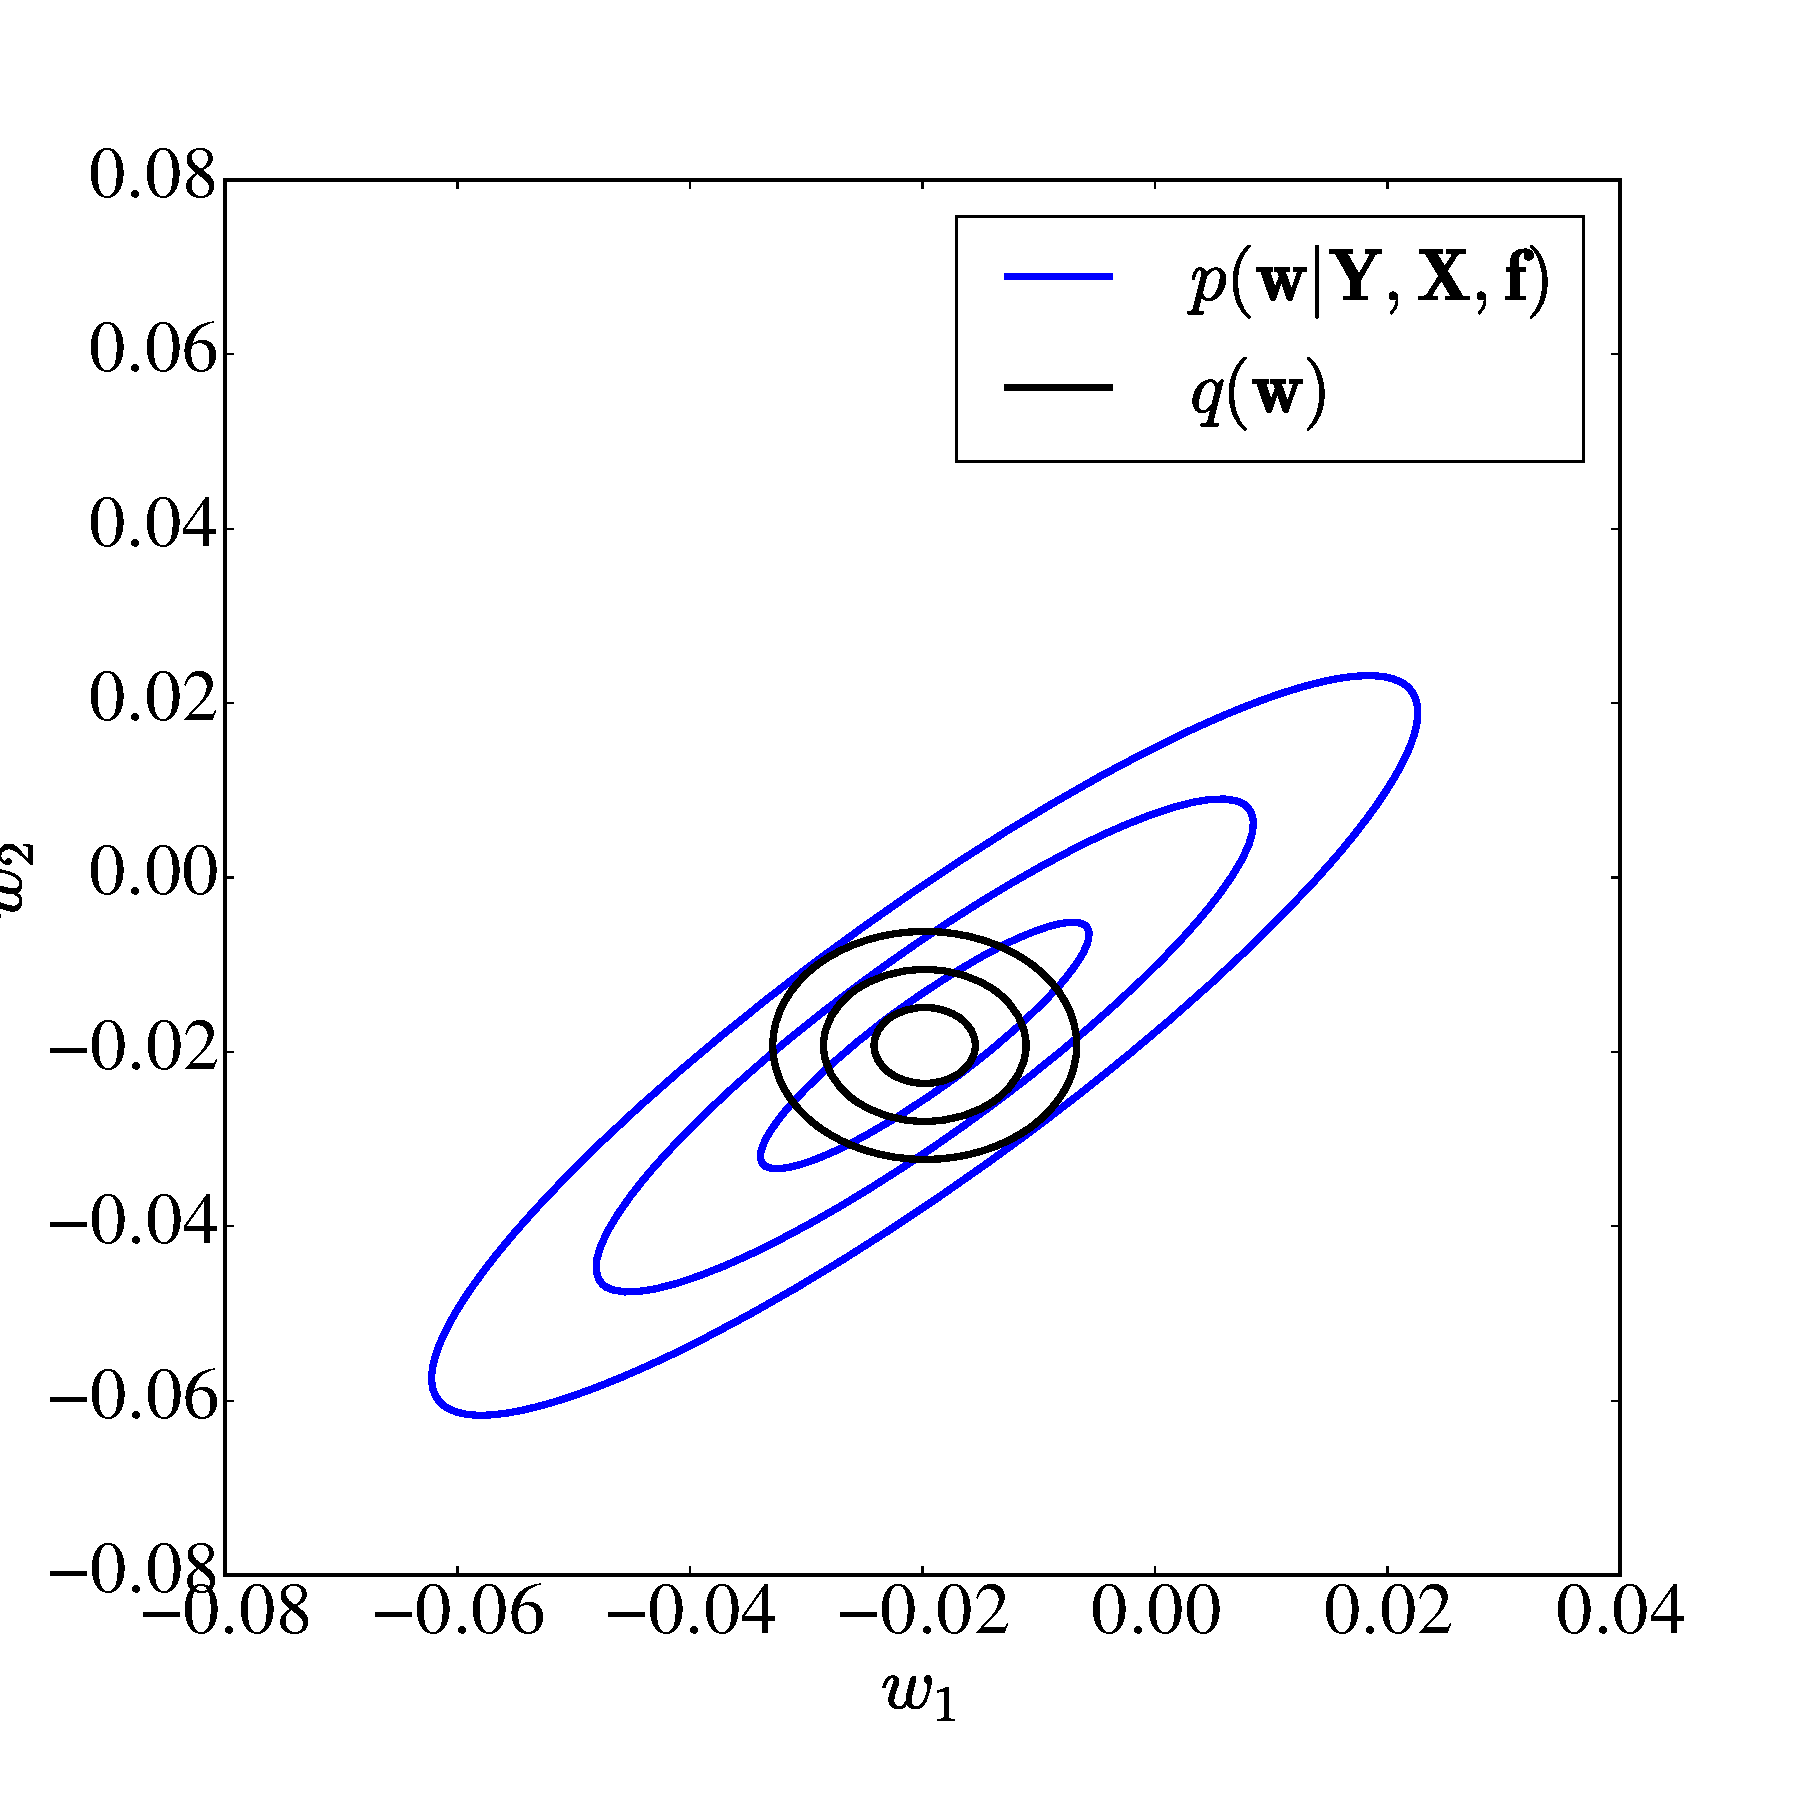
\includegraphics[width=0.8\textwidth]{mf.pdf}
\end{figure}
\end{center}

\end{column}%
\end{columns}

\end{frame}


\begin{frame}
\frametitle{ Graves, 2011}


\textbf{Априорное распределение:} $p(\mathbf{w}|\sigma) \sim \mathcal{N}(\boldsymbol{\mu}, \sigma \mathbf{I}).$\\
\textbf{Вариационное распределение:} $q (\mathbf{w}) \sim \mathcal{N}(\boldsymbol{\mu}_q, \sigma_q \mathbf{I}).$\\
Жадная оптимизация гиперпараметров:
\[
	\boldsymbol{\mu} = \hat{\mathsf{E}} \mathbf{w},
\quad
	\sigma = \hat{\mathsf{D}} \mathbf{w}.
\]

Прунинг параметра ${w}_i$ определяется относительной плотностью:
\[
	\lambda = \frac{q(\mathbf{0})}{q(\boldsymbol{\mu}_{i,q})}  = \text{exp}(-\frac{\mu_i^2}{2\sigma_i^2}).
\]
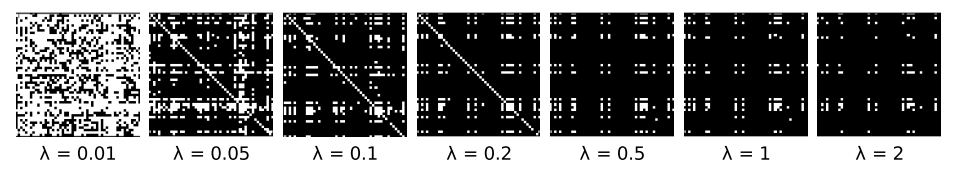
\includegraphics[width=\textwidth]{graves.png}
\end{frame}







\begin{frame}
\frametitle{ Louizos et. al, 2017}
\textbf{Априорное распределение} задается для каждого нейрона отдельно:
$p({w}_{ij}|\sigma) \sim \mathcal{N}(0, z), \quad p(z_i) \propto |z_i|^{-1}.$\\

$$p(\mathbf{w}, \mathbf{z}) \propto \prod_i \frac{1}{|z_i|} \prod_{j} \mathcal{N}(w_{i,j}|0,z_i^2).$$

\textbf{Вариационное распределение:} $q(\mathbf{z}) = \mathcal{N}(\boldsymbol{\mu^z}_q, \boldsymbol{\sigma^z}_q \mathbf{I}), \quad   q(\mathbf{w}) \sim \mathcal{N}(\boldsymbol{\mu}_q, \sigma_q \mathbf{I}).$\\


Прунинг нейронов $\mathbf{w}_i$ определяется величиной
\[
	\frac{\boldsymbol{\sigma^z}_{q,i}^2}{\boldsymbol{\mu^z}_{q,i}^2}.
\]
\end{frame}


\begin{frame}{Кросс-Валидация vs. Evidence: отбор признаков}
\begin{figure}
  \centering
  \subfloat[Кросс-валидация]{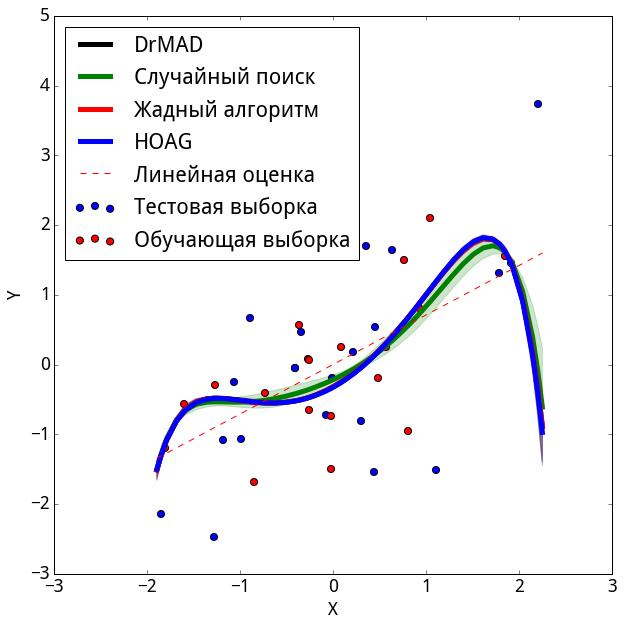
\includegraphics[width=0.42\textwidth]{poly_cv.png}} 
 \subfloat[Evidence]{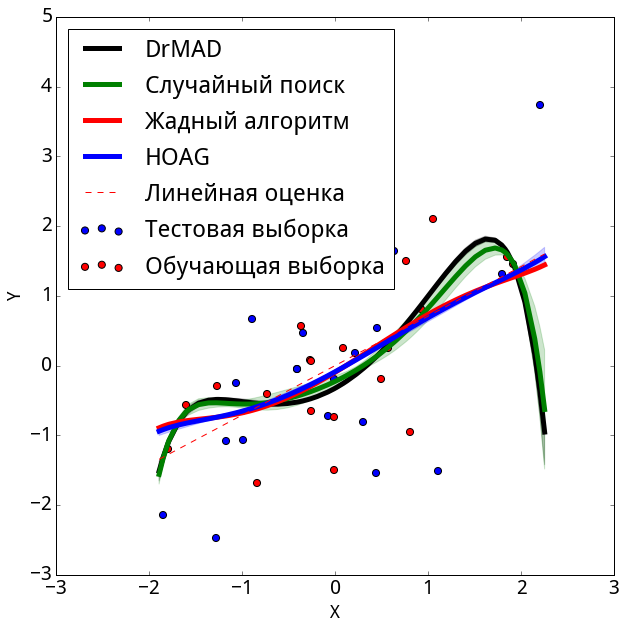
\includegraphics[width=0.42\textwidth]{poly_var.png}}
\label{fig:1}\qquad

\end{figure}
\end{frame}

\begin{frame}{Оператор оптимизации, Maclaurin et. al, 2015}
\begin{block}{Определение}
Назовем оператором оптимизации алгоритм $T$ выбора вектора параметров $\mathbf{w}'$  по параметрам предыдущего шага $\mathbf{w}$:
\[
	\mathbf{w}' = T(\mathbf{w}).
\]
\end{block}

\begin{block}{Определение}
Пусть $L$ --- дифференцируемая функция потерь. \\
Оператором градиентного спуска назовем следующий оператор:
\[
    T(\mathbf{w}) = \mathbf{w} - \gamma \nabla L(\mathbf{w}, \mathbf{y}, \mathfrak{D}).
\]
\end{block}


\end{frame}

\begin{frame}{Градиентный спуск для оценки правдоподобия}
Рассмотрим максимизацию совместного распределения параметров:
\[
    L =  -\text{log}~p(\mathfrak{D},\mathbf{w}|\mathbf{f}) = -\sum_{\mathfrak{D} \in \mathfrak{D}} \text{log}~p(\mathfrak{D}|\mathbf{w}, \mathbf{f}) p(\mathbf{w}|\mathbf{f})
\]
Проведем оптимизацию нейросети  из $r$ различных начальных приближений $\mathbf{w}_1, \dots, \mathbf{w}_r$ с использованием градиентного спуска:
\[
\mathbf{w}' = T(\mathbf{w}).
\]

Векторы параметров $\mathbf{w}_1,\dots,\mathbf{w}_r$ соответствуют некоторому скрытому распределению $q(\mathbf{w})$.

\end{frame}

\begin{frame}{Энтропия}
Формулу вариационной оценки можно переписать с использованием энтропии:
$$\text{log}~p(\mathfrak{D}|\mathbf{f}) \geq 
\int_{\mathbf{w}} q(\mathbf{w})\text{log}~\frac{p(\mathfrak{D},\mathbf{w}|\mathbf{f})}{q(\mathbf{w})}d\mathbf{w} = 
$$
$$
\mathsf{E}_{q(\mathbf{w)}}[\text{log~}p (\mathfrak{D}, \mathbf{w}| \mathbf{f})] - \mathsf{S}({q(\mathbf{w)}}),
$$
где $\mathsf{S}({q(\mathbf{w)}})$ --- энтропия:
$$
\mathsf{S}({q(\mathbf{w)}}) = - \int_{\mathbf{w}} q(\mathbf{w})\text{log}~q(\mathbf{w})d\mathbf{w}.  	
$$
\end{frame}




\begin{frame}{Градиентный спуск для оценки правдоподобия}
При достаточно малой длине шага оптимизации $\gamma$ разность энтропии на различных шагах оптимизации вычисляется как:
\[
\mathsf{S}(q'(\mathbf{w})) -  \mathsf{S}(q(\mathbf{w}))  \simeq  \frac{1}{r}\sum_{g=1}^r \bigl(-\gamma \text{Tr}[\mathbf{H}(\mathbf{w}'^g)] - \gamma^2 \text{Tr}[\mathbf{H}(\mathbf{w}'^g)\mathbf{H}(\mathbf{w}'^g)]  \bigr).
\]

Итоговая оценка на шаге оптимизации $\tau$:
$$
\text{log}~\hat{p}(\mathbf{Y}|\mathfrak{D}, \mathbf{f}) \sim \frac{1}{r} \sum_{g = 1}^r L(\mathbf{w}^g_\tau, \mathfrak{D}, \mathbf{Y})  + \mathsf{S}(q^0(\mathbf{w})) + \frac{1}{r}\sum_{b=1}^\tau\sum_{g=1}^r \bigl(-\gamma \text{Tr}[\mathbf{H}(\mathbf{w}_b^g)] - \gamma^2 \text{Tr}[\mathbf{H}(\mathbf{w}_b^g)\mathbf{H}(\mathbf{w}_b^g)]  \bigr),
$$
$\mathbf{w}_b^g$ --- вектор параметров старта $g$ на шаге $b$, $\mathsf{S}(q^0(\mathbf{w}))$ --- начальная энтропия.
\end{frame}
\begin{frame}{Переобучение,  Maclaurin et. al, 2015}
Градиентный спуск не минимизирует дивергенцию $\text{KL}(q(\mathbf{w})||p(\mathbf{w}| \mathfrak{D}))$. При приближении к моде распределения снижается оценка Evidence, что интерпретируется как переоубчение модели.

\begin{figure}
  \centering
  \subfloat[Схождение распределения к моде]{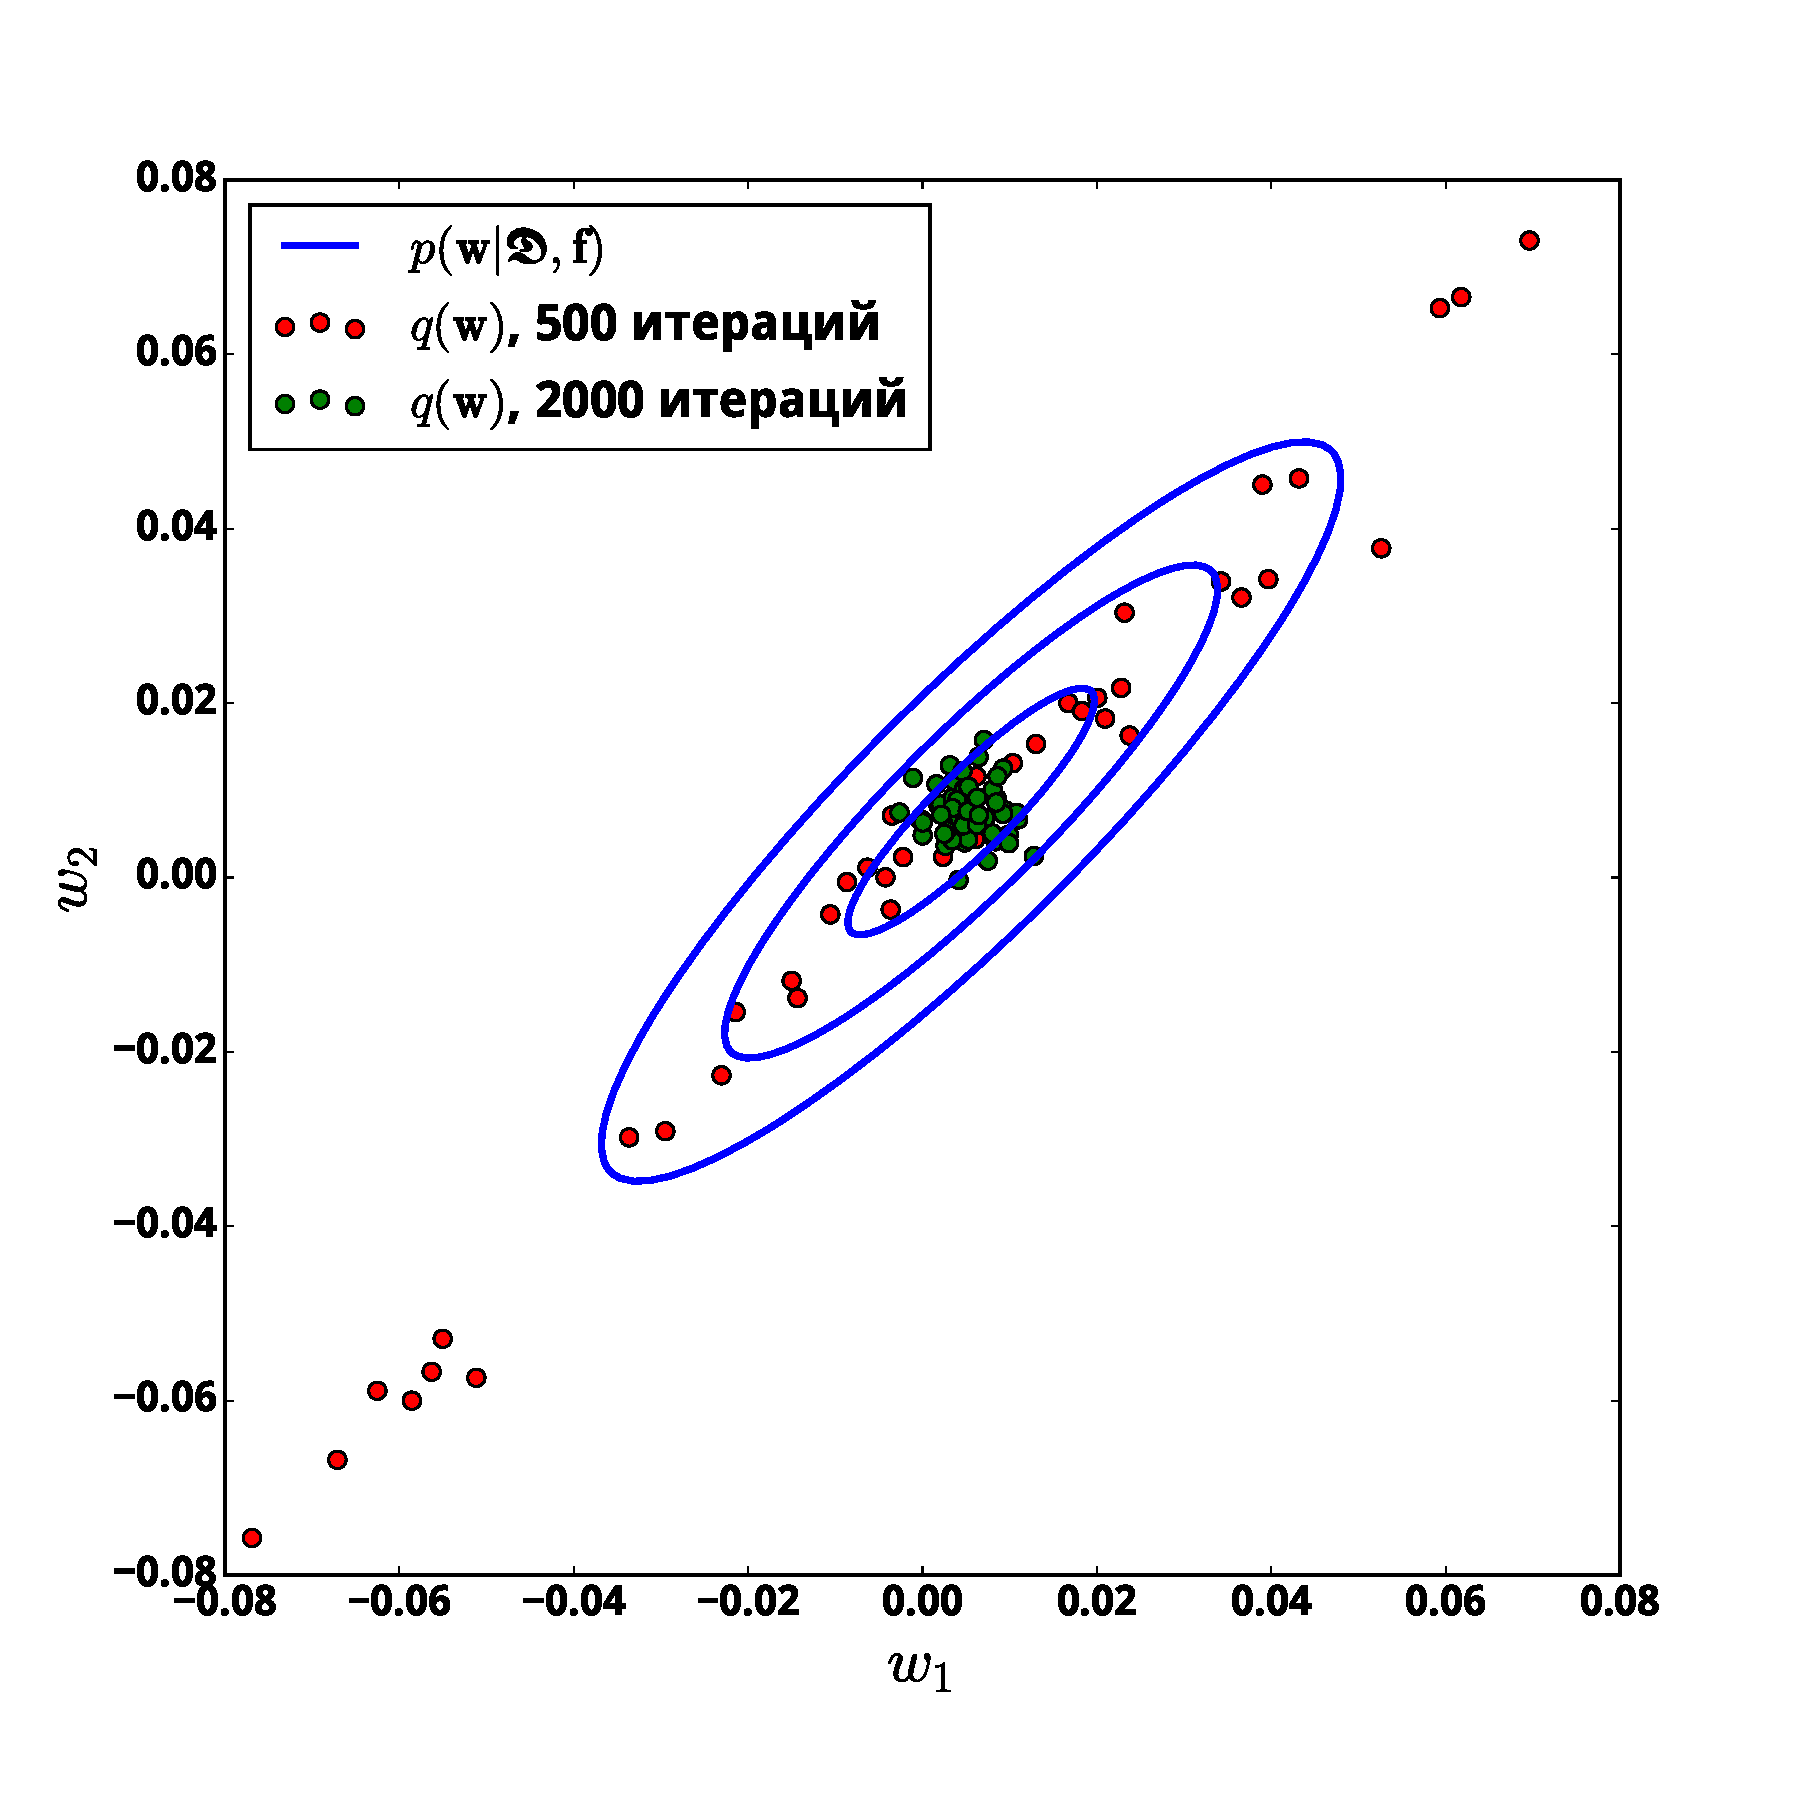
\includegraphics[width=0.35\textwidth]{sgd_estimate.pdf}} 
 \subfloat[Оценка начала переобучения]{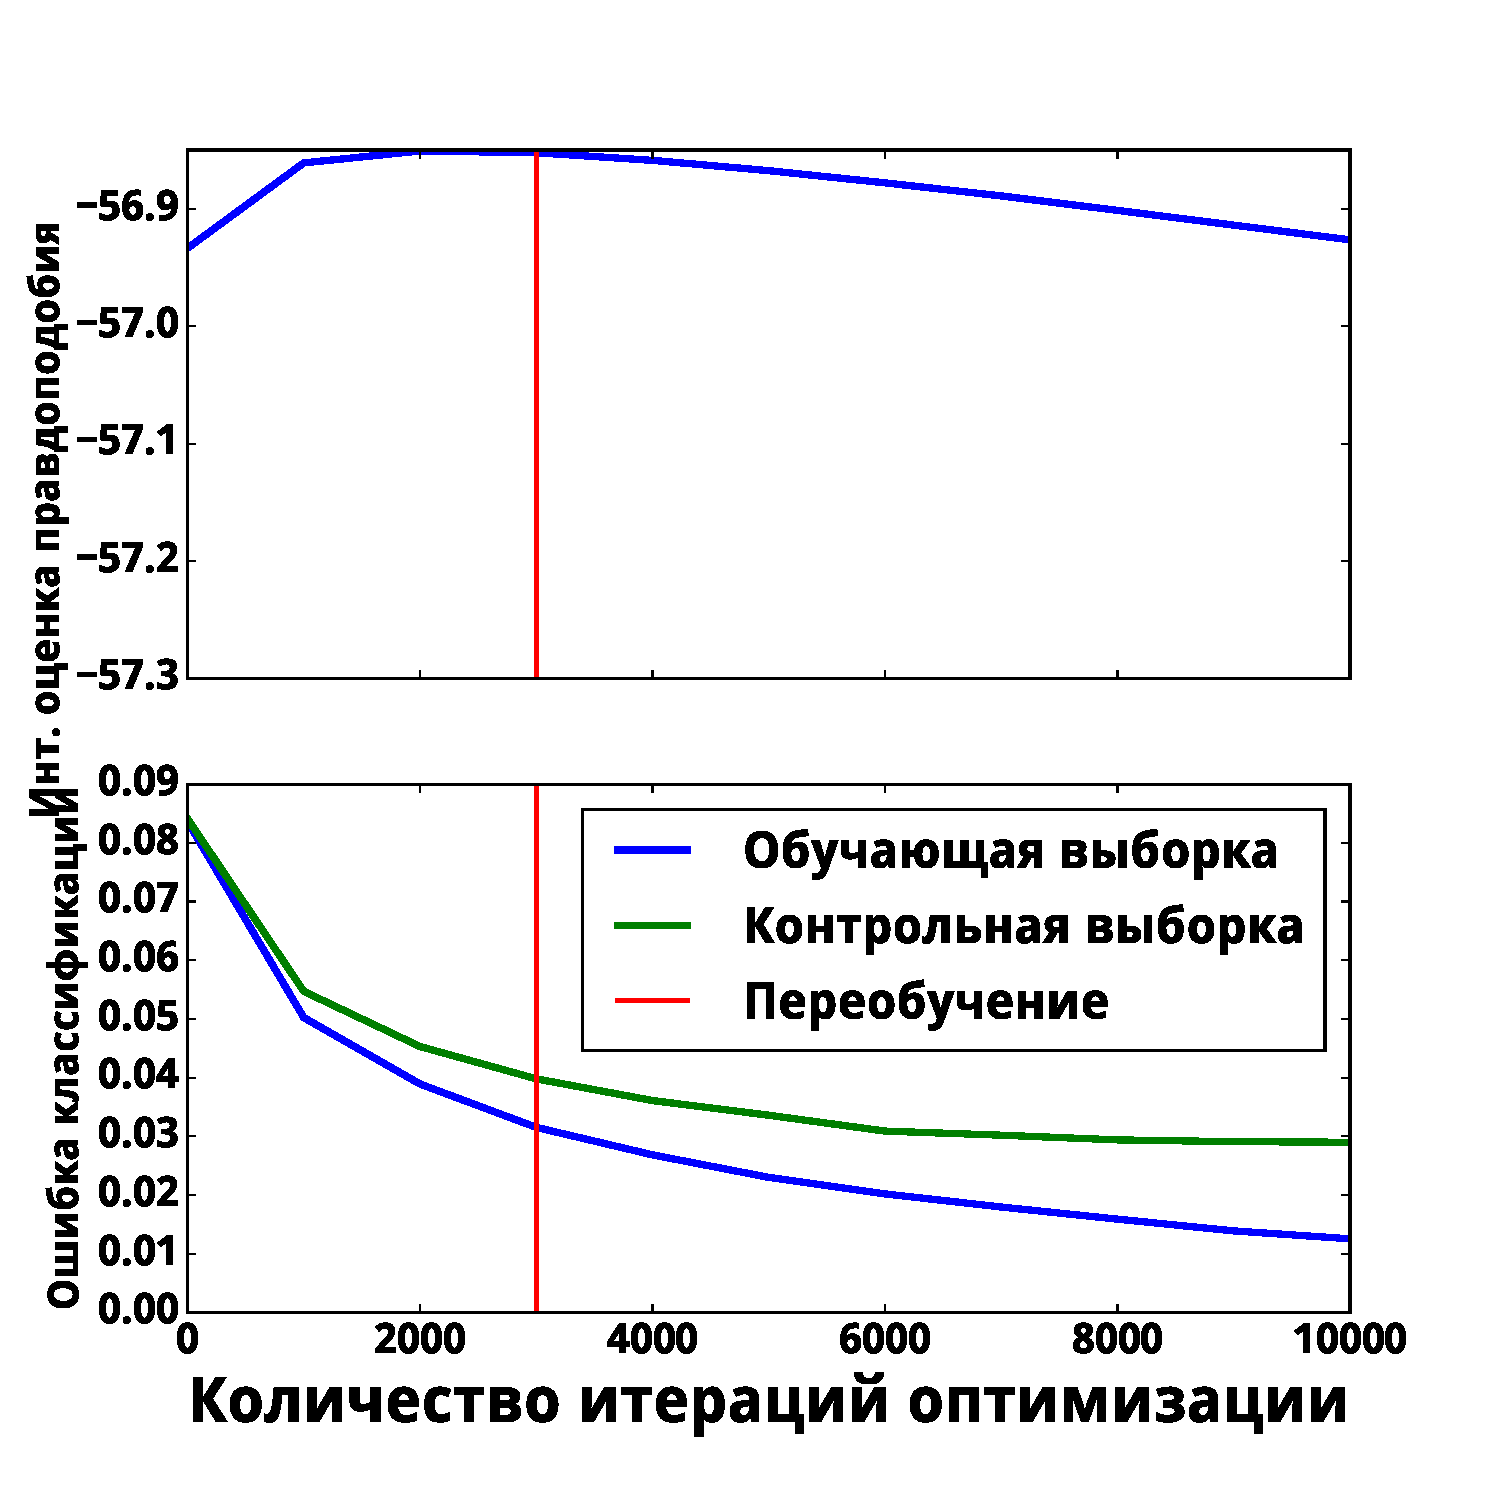
\includegraphics[width=0.35\textwidth]{sgd_show.pdf}}
\label{fig:1}\qquad
\end{figure}
\end{frame}

\begin{frame}
\frametitle{Стохастическая динамика Ланжевена}
Модификация стохастического градиентного спуска:
\[
	T(\mathbf{w})=\mathbf{w} -  \gamma \nabla (\text{log}p(\mathbf{w})+\frac{m}{\hat{m}}\text{log}p(\hat{\mathfrak{D}}|\mathbf{w}))  \textcolor{red}{+ \epsilon, \quad   \textcolor{red}{\epsilon \sim  \mathcal{N}({0},{\frac{\gamma}{2}})}}
\]
где $\hat{m}$ --- размер подвыборки,  $\hat{\mathfrak{D}} \subset \mathfrak{D}$ --- подвыборка, шаг оптимизации $\gamma$ изменяется с количеством итераций:
\[
	\sum_{\tau=1}^\infty \gamma_\tau = \infty, \quad \sum_{\tau=1}^\infty \gamma_\tau^2 < \infty.
\]
\textbf{Утверждение~[Welling, 2011].} Распределине $q^\tau(\mathbf{w})$ сходится к апостериорному распределению $p(\mathbf{w} | \mathfrak{D},\mathbf{f})$.


Изменение энтропии с учетом добавленного шума:
\[
\hat{\mathsf{S}}\bigl(q^\tau(\mathbf{w})\bigr)   \geq \frac{1}{2}|\mathbf{w}|\text{log}\bigl(\text{exp}(\frac{2\mathsf{S}(q^\tau(\mathbf{w}))}{|\mathbf{w}|}) + \text{exp}(\frac{2\mathsf{S}( \epsilon)}{|\mathbf{w}|})\bigr).
\]

\end{frame}



\begin{frame}
\frametitle{Стохастическая динамика Ланжевена}
Распределения параметров после 2000 итераций:
\begin{figure}[h]
\centering
\subfloat[]{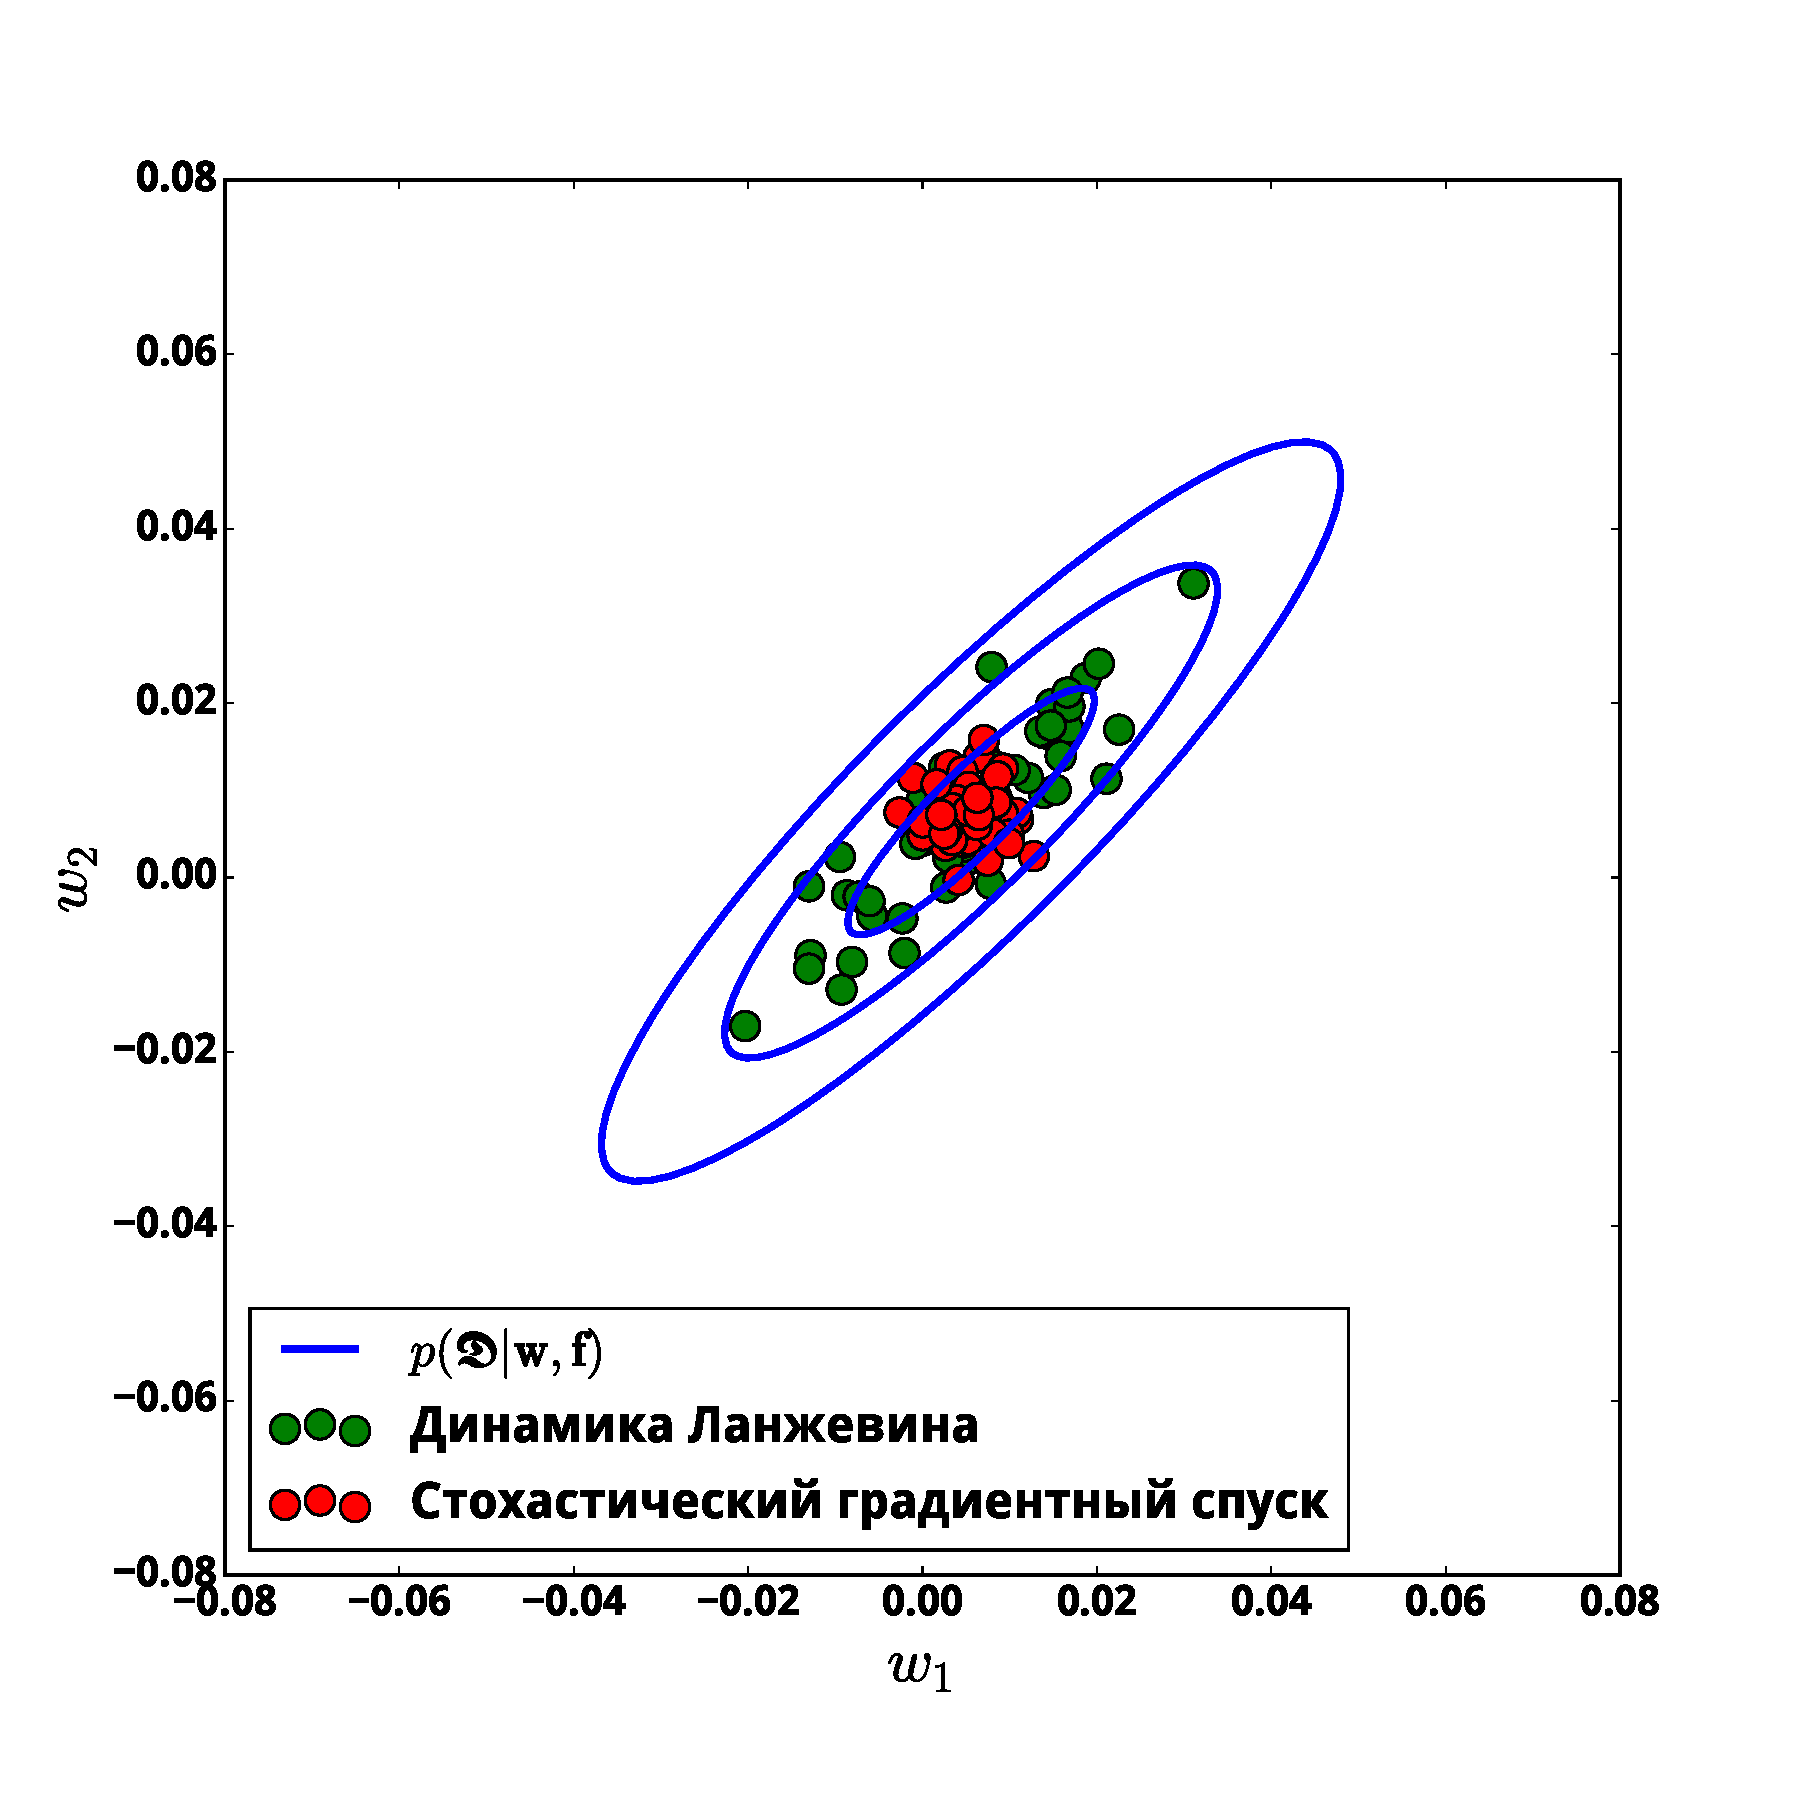
\includegraphics[width=0.45\textwidth]{./langevin_estimate.pdf}}
\end{figure}

\end{frame}

\begin{frame}{Выбор константы регуляризации}
Выборка MNIST, 50 нейронов на скрытом слое.

\begin{figure}
  \centering
  \subfloat[Кросс-валидация]{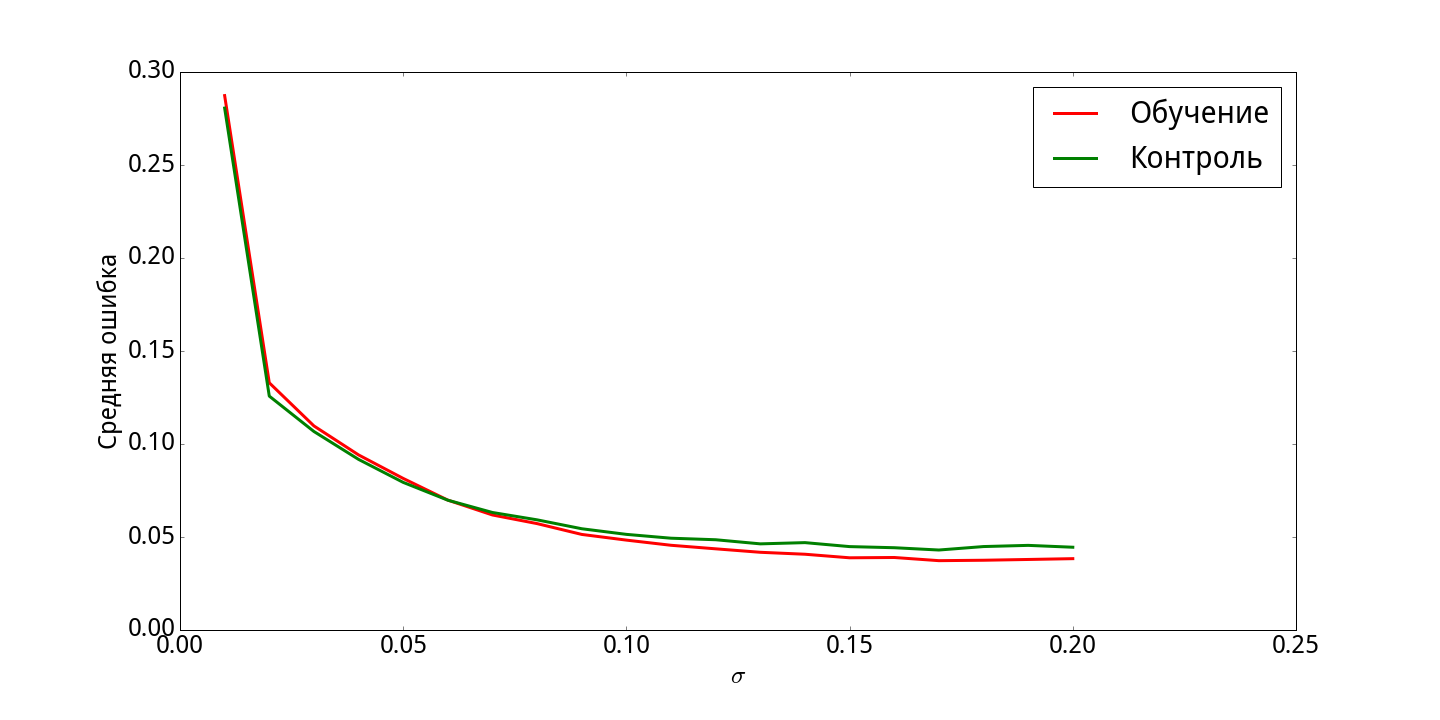
\includegraphics[width=0.5\textwidth]{sgd2.png}} 
 \subfloat[Оценка Evidence]{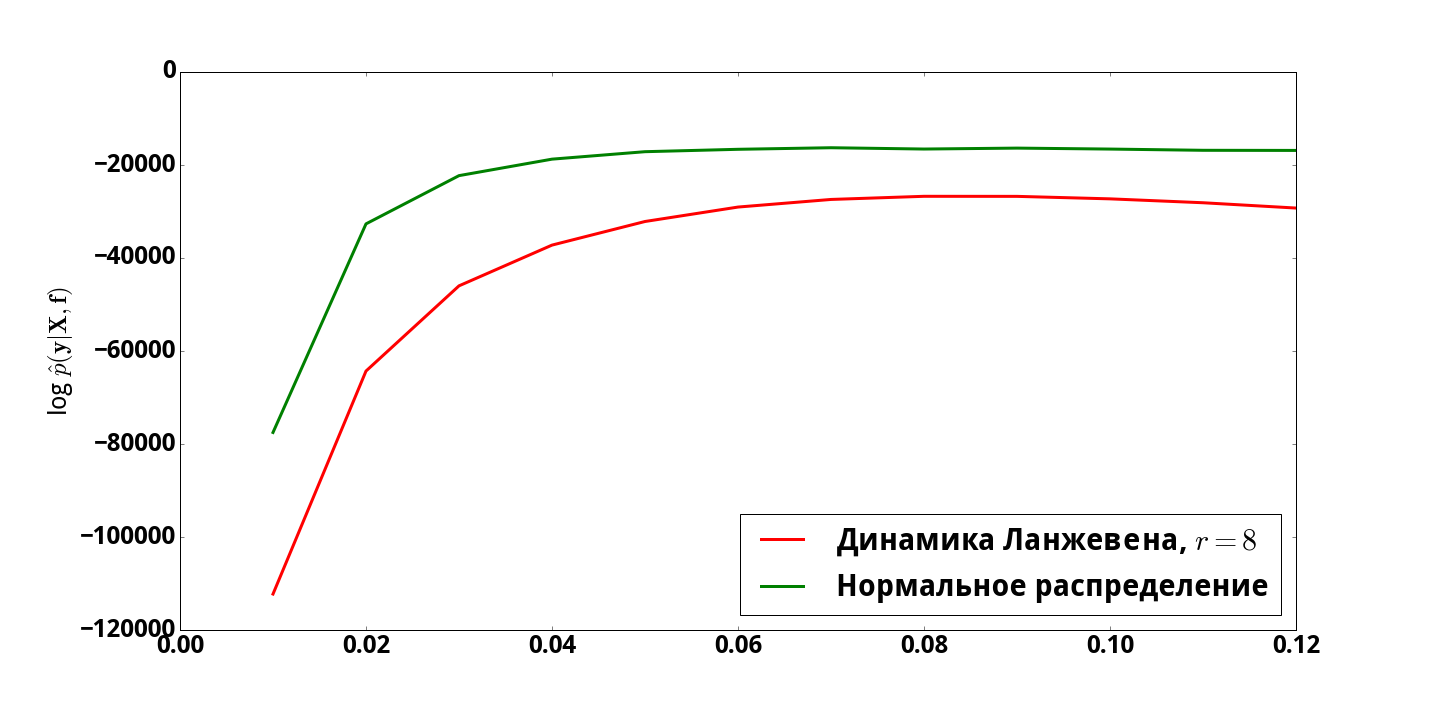
\includegraphics[width=0.5\textwidth]{mnist_evidence2.png}}
\label{fig:1}\qquad
\end{figure}

\end{frame}


\begin{frame}{Качество моделей при возмущении параметров}

\begin{figure}
  \centering
  \subfloat[Boston: 3-слойная нейросеть]{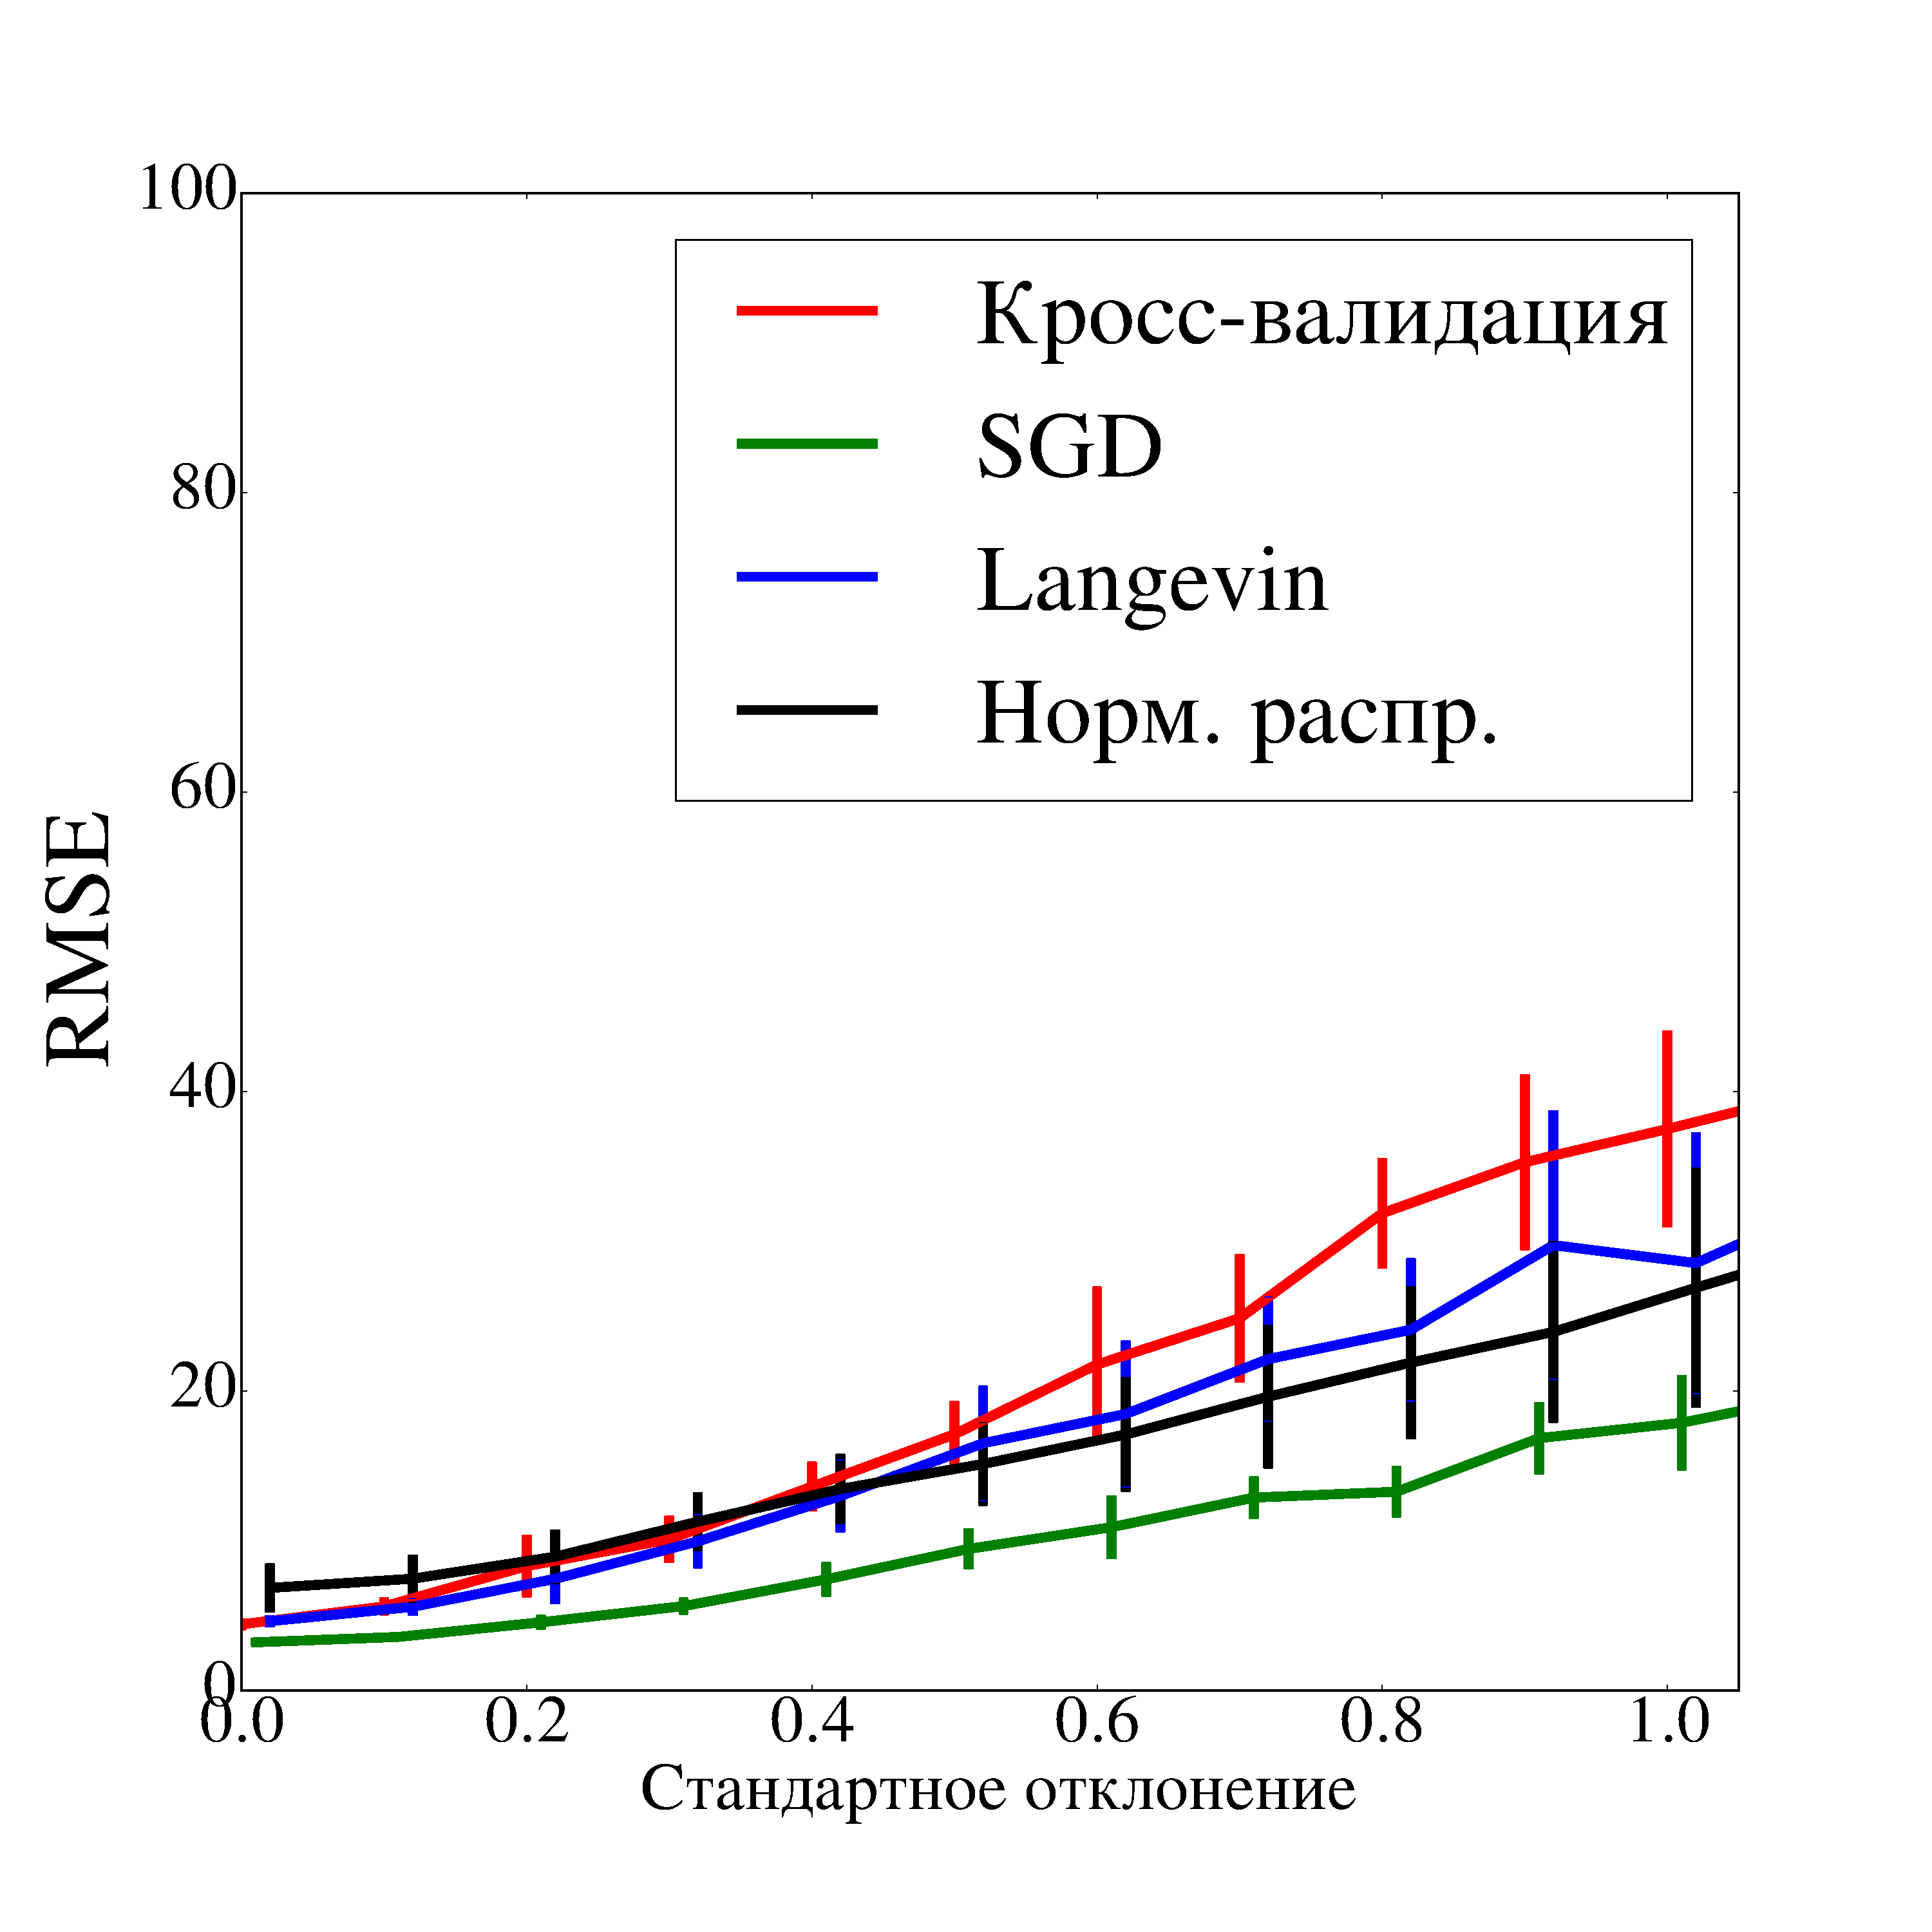
\includegraphics[width=0.42\textwidth]{rmse_data.pdf}} 
 \subfloat[MNIST (50-dim PCA): 3-слойная нейросеть]{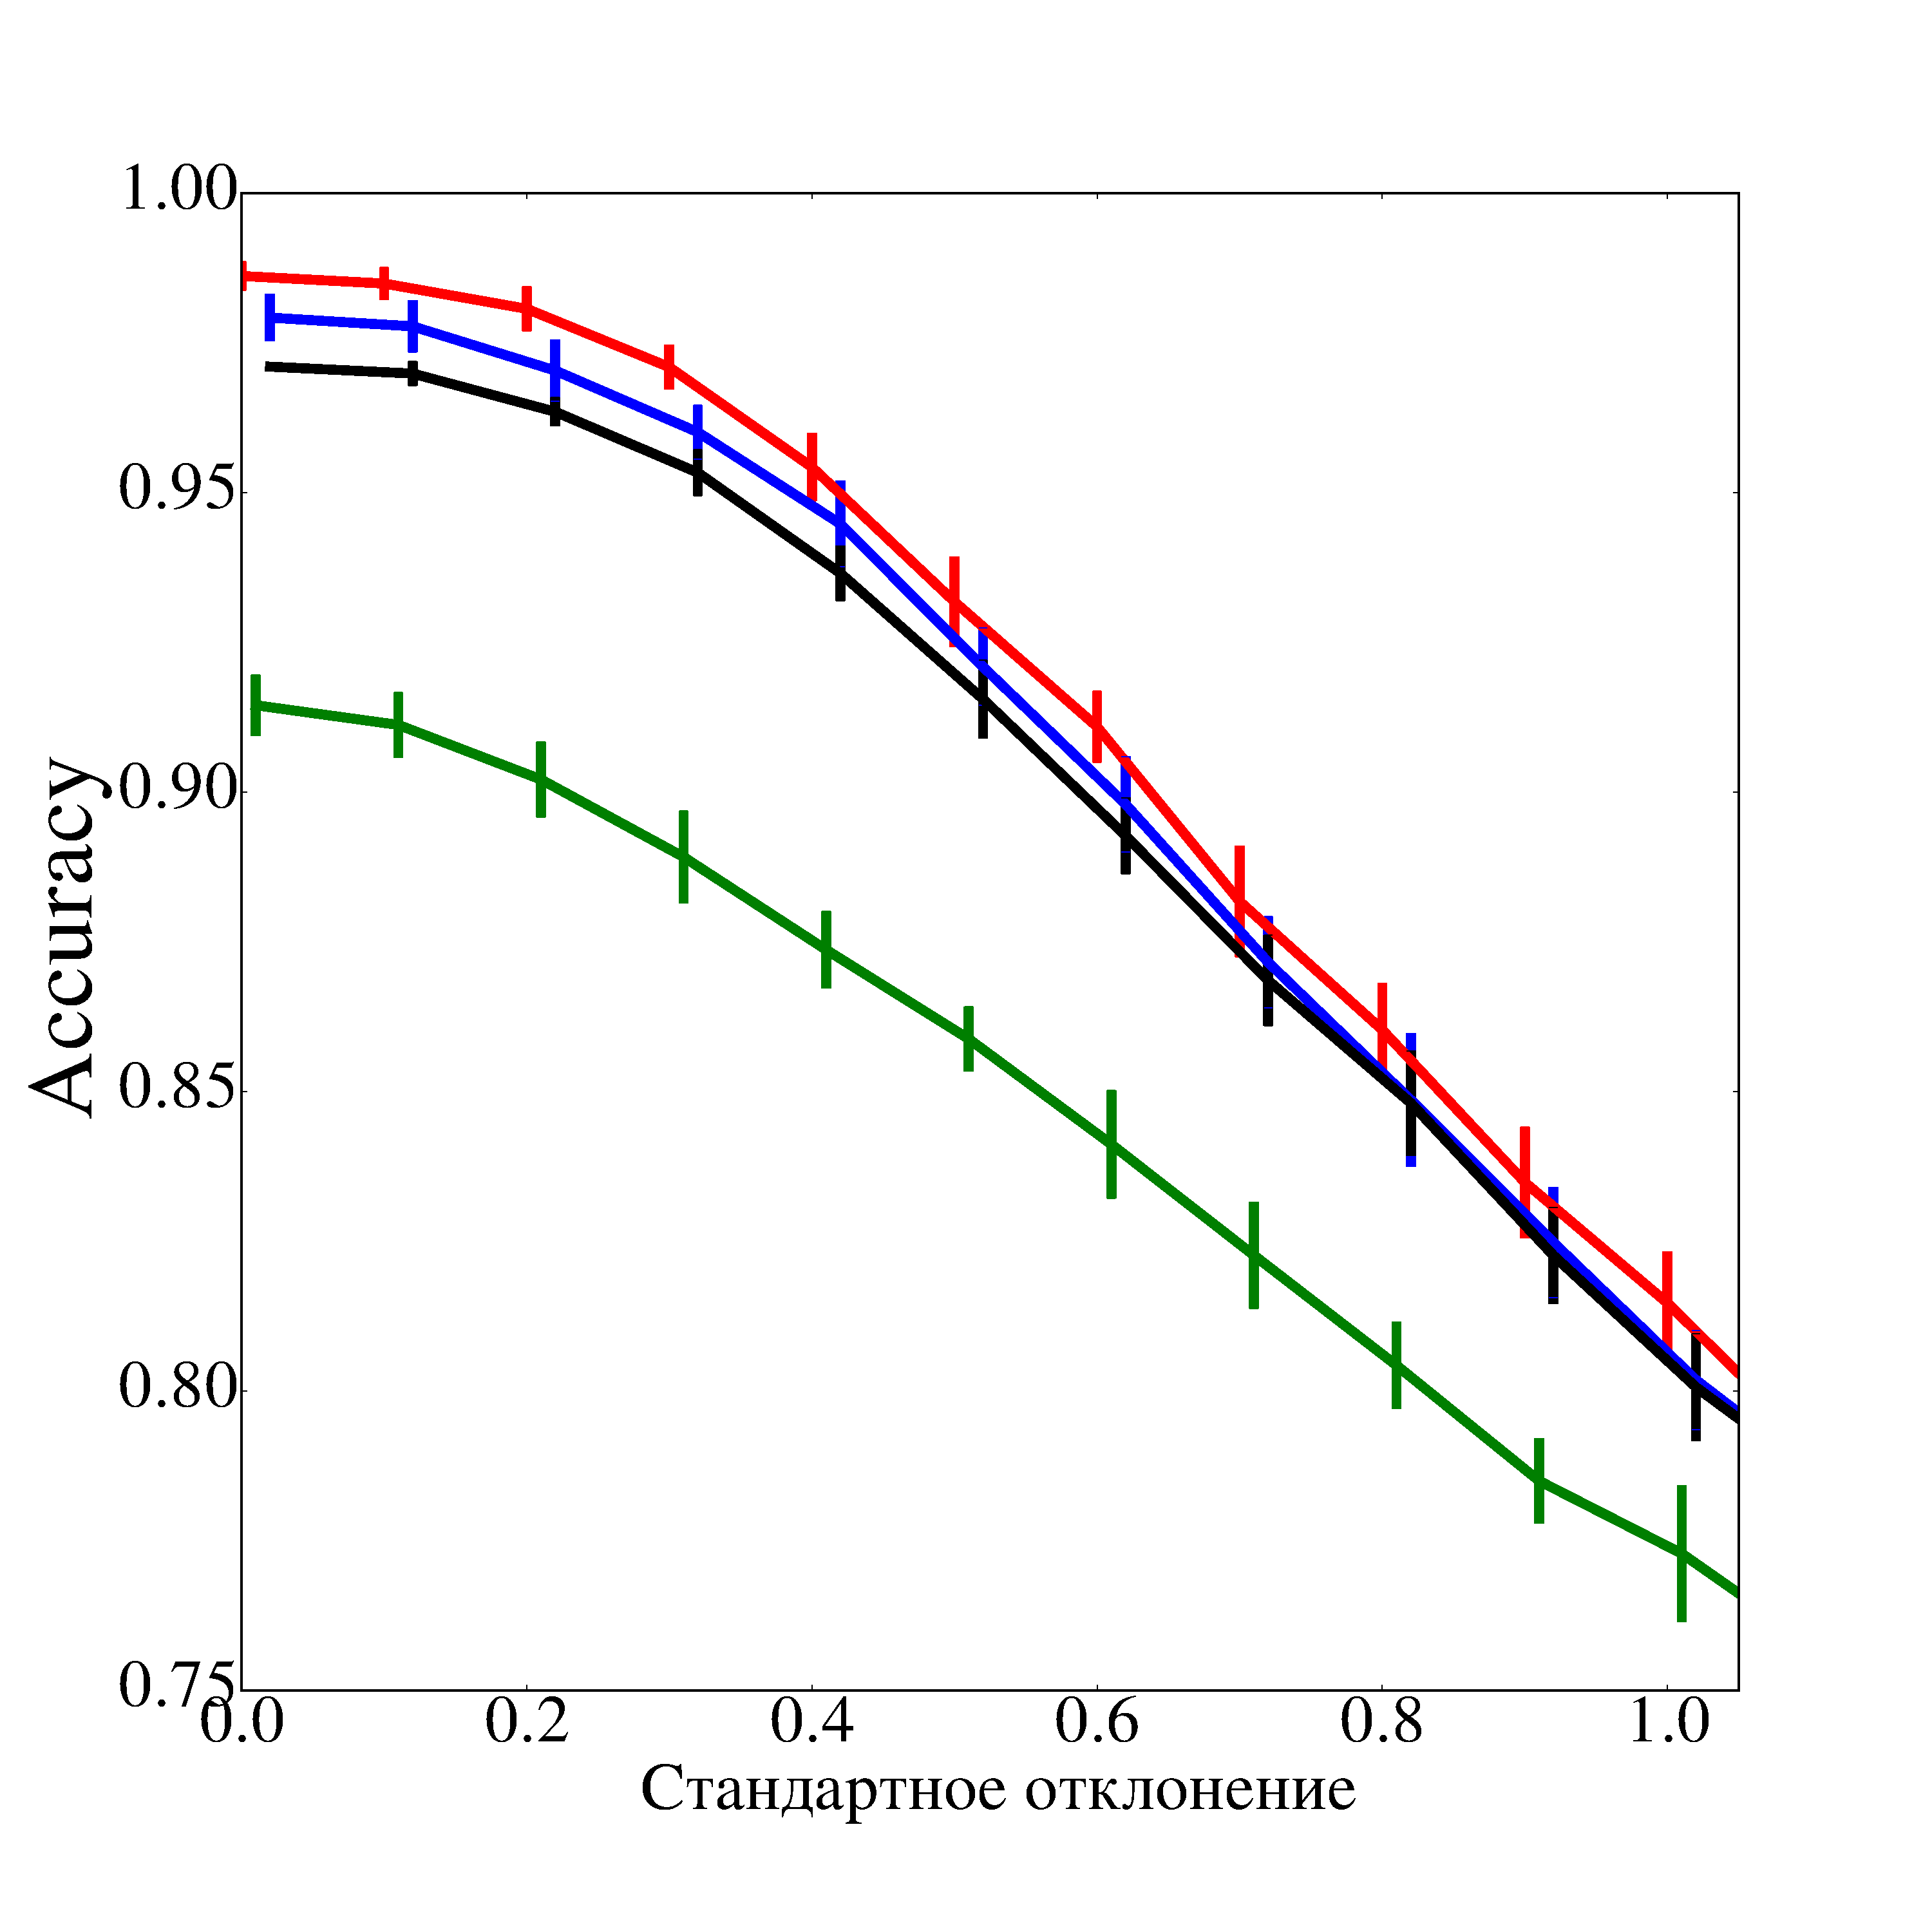
\includegraphics[width=0.42\textwidth]{acc_data.pdf}}
\label{fig:1}\qquad

\end{figure}

\end{frame}

\begin{frame}
\frametitle{Используемые материалы}
\begin{enumerate}
\item David J. C. MacKay, Information Theory, Inference \& Learning Algorithms, 2003
\item Peter Grunwald, A tutorial introduction to the minimum description length principle, 2004 
\item Christopher Bishop, Pattern Recognition and Machine Learning, 2006
\item Welling W., Teh Y.W., Bayesian Learning via Stochastic Gradient Langevin Dynamics, 2011
\item Alex Graves, Practical Variational Inference for Neural Networks, 2011
\item Maclaurin D., Duvenaud D., Adams R.P., Early Stopping is Nonparametric Variational Inference, 2015
\item Kuznetsov M.P., Tokmakova A.A., Strijov V.V. Analytic and stochastic methods of structure parameter estimation, 2016
\item Louizos C., Ullrich K., Welling M., Bayesian Compression for Deep Learning, 2017
\item Zoph B., Vasudevan V., Shlens J., Le Q. V., Learning Transferable Architectures for Scalable Image Recognition, 2017
\item Бахтеев О.Ю., Стрижов В.В., Выбор моделей глубокого обучения субпотимальной сложности, 2018
\end{enumerate}
\end{frame}

\end{document}

